%\documentclass[a4paper]{report}
\documentclass[a4paper]{report}

%BEFORE SUBMISSION DO THESE:
% * deactivate all \includeonly
% * ensure \doneit set to nothing
% * ensure numbering CONTINUOUS from title page on through
% * activate the includes of license, ack, etc
% * check through for question mark errors in render
% * make sure the bibliog doesn't have ugly urls in

\usepackage[left=40mm,right=30mm]{geometry}
\usepackage[printonlyused]{acronym}
\usepackage{ifdraft}
\usepackage{mathtools}
\usepackage{braket}
\usepackage{tgtermes} % font
\usepackage{comment}
\usepackage{amssymb}
\usepackage{bm}%bold math symbols
\usepackage{rotating}
\usepackage{hyperref}
\usepackage{textcomp}
\usepackage{gensymb} % degree symbol etc
\usepackage{subfig} % apparently subfig is the one to use not subfigure
\usepackage{appendix}
\usepackage{tipa}
\usepackage{clrscode}
\usepackage{setspace}
\usepackage[absolute]{textpos}
\usepackage[super,sort&compress,comma]{natbib} 
%\makeatletter %\renewcommand\@biblabel[1]{#1.} %\makeatother %uncomment these for "1." style bib
\usepackage{titlesec}
\usepackage{siunitx}
\usepackage{notoccite} %stops citations in captions ruining everything
\usepackage{float}
\usepackage[version=4]{mhchem} %chemistry formulae
\usepackage{epigraph}
\titleformat{\chapter}[block]
  {\normalfont\huge\bfseries}{\thechapter}{1em}{\huge}
\titlespacing*{\chapter}{0pt}{*0}{2em}
\usepackage{fancyhdr}
\pagestyle{fancy}
\fancyhf{}
\renewcommand{\chaptermark}[1]{\markboth{\thechapter{} #1}{}}
\lhead{\leftmark}
\chead{}
\lfoot{}
\cfoot{}
\rhead{\thepage}

\def\szero{S$_{0}$}
\def\sone{S$_{1}$}
\def\stwo{S$_{2}$}
\def\sthree{S$_{3}$}
\def\pipistar{$\pi\pi^{\ast}$}
\def\pistar{$\pi^{\ast}$}
\def\npistar{$n\pi^{\ast}$}
\def\Estar{E$^\ast$}
\def\Kstar{K$^\ast$}
\DeclareTextCompositeCommand{\r}{OT1}{A}{% Angstrom!
  \leavevmode\vbox{%
    \offinterlineskip
    \ialign{\hfil##\hfil\cr\char23\cr\noalign{\kern-1.15ex}A\cr}%
  }%
}
\begin{document}

\setlength{\TPHorizModule}{200mm} 
\setlength{\TPVertModule}{100mm} 
\textblockorigin{61mm}{19mm}


%%%%% thanks alex mclean for super-useful onscreen reading tip:
%\usepackage[top=0.1in, bottom=0.1in, left=0.3in, right=0.3in, paperwidth=11in, paperheight=7in]{geometry} % activate for ONSCREEN reading shape AT HOME
%\usepackage[top=0.1in, bottom=0.1in, left=0.3in, right=0.3in, paperwidth=11in, paperheight=8.5in]{geometry} % activate for ONSCREEN reading shape AT WORK

\onehalfspace{}

% activate the appropriate shortcut, whether or not to show this in titles
%	\providecommand{\doneit}{DONE: }
%	\providecommand{\doneit}{}

% Some specific notations used:
\providecommand{\OT}[1]{\operatorname{\Theta}\bigl(#1\bigr)}
\providecommand{\OOm}[1]{\operatorname{\Omega}\bigl(#1\bigr)}
%\newcommand{\concat}{{\,++\,}}

% numbering starts from here:
\pagenumbering{arabic}

% titlepage stuff
\title{\huge
\textbf{Modelling of Photophenomena\\ in Condensed Phase}}
\author{Michael Dommett \\
%\\
%PhD Thesis\\
\\
School of Biological and Chemical Sciences\\
Queen Mary University of London\\
\\
Submitted in partial fulfillment of the requirements\\ of the Degree of Doctor of Philosophy}

\date{2018}


\maketitle
%%%% qmul rules say abstract must be FIRST after title page

\begin{abstract}

This is the abstract.

\end{abstract}  

\setcounter{page}{3}

\chapter*{Licence}

This work is copyright \copyright \ 2016 Your Name, and is licensed under TO BE DECIDED - CHOOSE YOUR OWN OR USE CUURENT UNIVERSITY GUIDELINES the Creative Commons Attribution-Share Alike 3.0 Unported 
Licence. To view a copy of this licence, visit \\
\url{http://creativecommons.org/licenses/by-sa/3.0/} \\
or send a letter to Creative Commons, 171 Second Street, Suite 300, San Francisco, California, 94105, USA.

\begin{center}

%	\includegraphics [width =1cm]  {images/cc}
%	\includegraphics [width =1cm]  {images/by}
%	\includegraphics [width =1cm]  {images/sa}
    
\end{center}
\chapter*{Acknowledgements}
\chapter*{}
\renewcommand{\epigraphsize}{\large}
\setlength{\epigraphwidth}{0.8\textwidth}
\renewcommand{\epigraphflush}{center}
\renewcommand{\epigraphrule}{0pt}
\epigraph{\textit{Uncertainty is an uncomfortable position. But certainty is an absurd one.}}{Votaire}

\listoffigures
\listoftables
\chapter*{List of abbreviations}
\begin{acronym}[OLED]
\acro{OLED}{organic light-emitting diode}
\acro{AIE}{aggregation induced emission}
\acro{ACQ}{aggregation caused quenching}
\acro{CT}{charge-transfer}
\acro{EQE}[$\eta$\textsubscript{QE}]{external quantum efficiency}
\acro{TICT}{twisted intramolecular charge transfer}
\acro{RIR}{restriction of intramolecular rotation}
\acro{RIV}{restriction of intramolecular vibrations}
\acro{RIM}{restriction of intramolecular motions}
\acro{TPE}{tetraphenylethene}
\acro{ESIPT}{excited state intramolecular proton transfer}
\acro{GSIPT}{ground state intramolecular proton transfer}
\acro{HBT}{2-(2-hydroxyphenyl)benzothiazole}
\acro{NIR}{near-infrared}
\acro{HC}[\textbf{HC}]{2'-hydroxychalcone}
\acro{HP}[\textbf{HP}]{2-hydroxyphenylpropenone}
\acro{MM}{molecular mechanics}
\acro{DFT}{density functional theory}
\acro{HF}{Hartree-Fock}
\end{acronym}

\tableofcontents
\chapter{Luminescent Organic Materials}
\label{chapter: luminscent organic materials}
%%%%%%%%%%%%%%%%%%%%%%%%%%%%%%
\section{Introduction}\label{section: lom introduction}
%%%%%%%%%%%%%%%%%%%%%%%%%%%%%%
Luminescent organic molecules are used in numerous biological and technological applications. In aqueous solution they are used extensively in biological imaging, probing, and detection. Deposited as thin films and aggregates, they represent the next generation of organic optoelectronics, where availability and low cost of starting materials, straightforward syntheses, and lightweight, flexible devices are attractive features. Perhaps most importantly, the luminescent response of molecular organic systems can be tuned with relative ease compared to their inorganic counterparts.

Since the discovery of electromluminescence in the 1960s, intensive efforts in academia and industry have delivered considerable progress in the field of organic electronics, leading to  the development of applications such as field-effect transistors, photovoltaic cells, optical memory devices, and single-crystal lasers.\cite{Ostroverkhova2016} The most prominent success story are certainly \acp{OLED}, which have already reached market adoption for lighting and display purposes. However, in many areas organic systems suffer from low efficiencies, trial-and-error optimisation, and decreased performance in aggregated form versus solution. 
To advance, there must be control over both the supermolecular structure of the material and the electronic structure of the  molecules within. Unfortunately neither of these properties exist in isolation, and the interplay between them must also be intimately understood, which somewhat complicates matters. Of these contributing factors, it is the electronic structure and its relationship with the environment which are of interest in this work. The luminescent response of molecules can change drastically from one medium to another, whether in the gas phase, as a solution, aggregated as clusters, or in molecular crystals. Understanding the interplay between the luminophore and its environment is crucial for designing more efficient materials from first principles. 

To this end, this work approaches the problem using theoretical chemistry methods to investigate organic compounds exhibiting \ac{AIE}. AIE-active compounds are non-emissive in dispersed media, but undergo a switch-on of luminescence, typically in the form of fluorescence, upon aggregation. Since technological applications require a thin-film or solid-state layer, AIE has attracted considerable interest as a pathway to overcome the common effect of \ac{ACQ}, hitherto a major obstacle in the development of organic luminophores. In this chapter the problem of \ac{ACQ} shall be introduced, followed by an examination of the AIE phenomenon through analysis of typical structures, mechanistic interpretations, before introducing the systems under investigation.
%%%%%%%%%%%%%%%%%%%%%%%%%%%%%%
\section{Aggregation Caused Quenching}\label{section: lom ACQ}
%%%%%%%%%%%%%%%%%%%%%%%%%%%%%%
\subsection{Molecular Stacking}
Photoinduced luminescence occurs after chromophores with $\pi$-conjugation, typically in the form of aromatic moieties, absorb light in the \ac{UV} or visible region of the electromagnetic spectrum. In good solvents or dilute concentration, fluorescence will usually follow, although the presence of metals or second row elements can allow phosphorescence via intersystem crossing. Upon aggregation with increased concentration, or crystallisation, the fluorescence is often reduced or quenched completely. 

In 1954, photochemisty pioneer Theodor F\"{o}rster elegantly showed that the fluorescence of pyrene is shifted and weakened with increasing concentration (Figure \ref{figure: Forster_Spectra}).\cite{Forster1954,Forster1969} As the concentration increases, a new fluorescent species is formed and the original band loses intensity. The new band at longer wavelength is a result of the formation of excited dimers, or \textit{excimers}. The presence of aromatic rings in conventional luminophores leads to intermolecular $\pi$-$\pi$ interactions and the formation of dimers. In F\"{o}rster's pyrene example, where the spectra of differing concentrations are measured using the same incident wavelength, the single intersecting point shows that the spectrum consists of only two features. Since the absorption spectrum is unchanged in the concentration range, the arising band can be ``attributed to an associate that exists only in the excited electronic state, i.e. to an excimer."\cite{Forster1969}
\begin{figure}[H]
\centering
  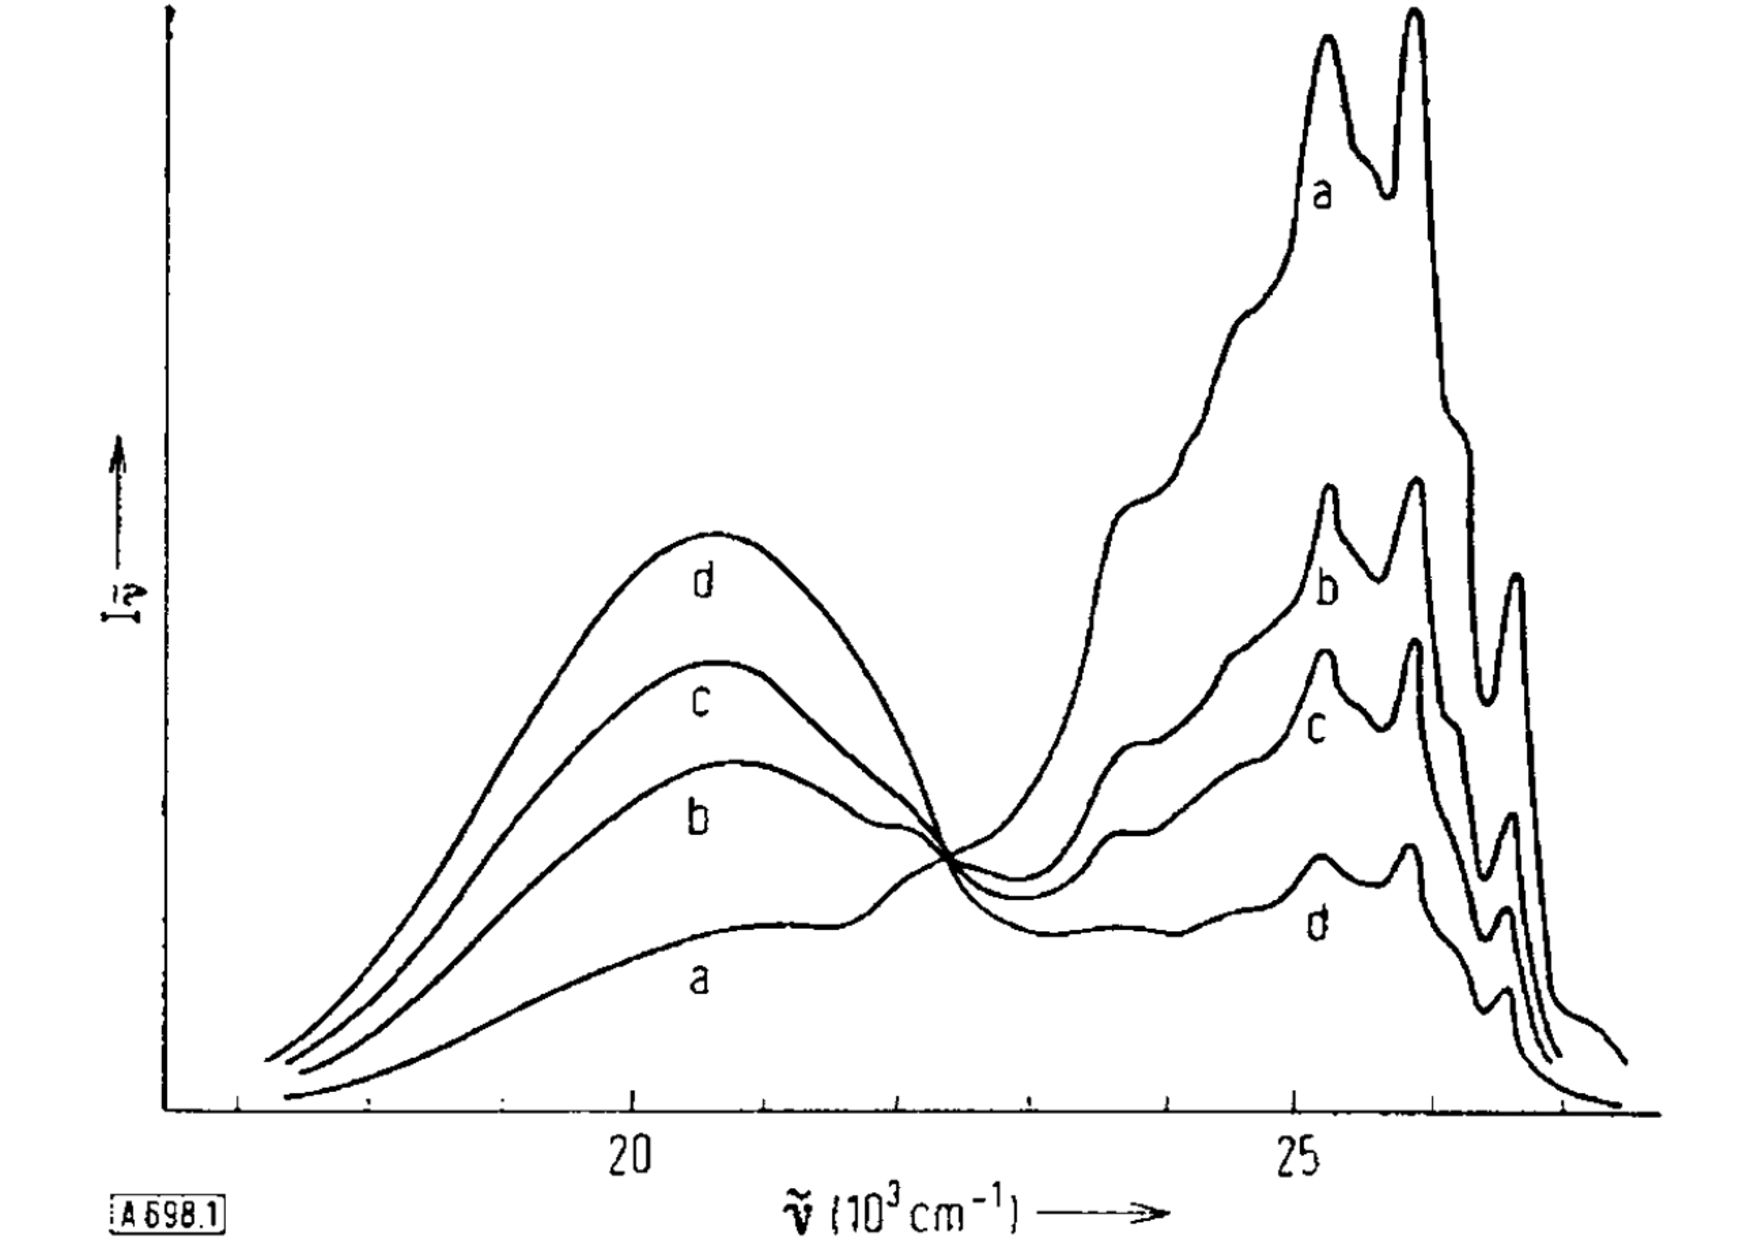
\includegraphics[width=0.6\linewidth]{1Intro/Forster_Spectra.pdf}
  \caption[Fluorescence spectrum of pyrene]{Fluorescence spectrum of pyrene (in n-heptane, 20\degree{}C) at different concentrations: a) \SI{5.0e-5}, b) \SI{1.8e-4}, c) \SI{3.1e-4}, d) \SI{7.0e-4}{mol L^{-1}}. Reprinted from ref.~\citenum{Forster1969} with permission of Wiley-VCH.}
  \label{figure: Forster_Spectra}
\end{figure}
The supermolecular alignment of aromatic groups is commonly termed $\pi$-stacking or $\pi$-$\pi$ interactions in the chemical literature. However, this labelling can be slightly misleading and even inaccurate.\cite{Grimme2008,Martinez2012} Stefan Grimme argues that a specific $\pi$-$\pi$ interaction arises only in large, polyaromatic groups as a result of increased dispersion in specific orientations.\cite{Grimme2008} Meanwhile, a thorough review of experimental and theoretical literature by Martinez and Iverson found a lack of the face-centred stacking of aromatic groups which would maximise overlap of aromatic $\pi$ clouds.\cite{Martinez2012} They argue that the terms $\pi$-stacking and $\pi$-$\pi$ interactions are misnomers since they incorrectly imply the ubiquity of face-face stacking motifs. Typical stacking motifs are shown in Figure \ref{figure: Benzene_Stacking}, where parallel displacement tempers the unfavourable electrostatic interaction and reduces the Pauli exchange repulsion, with the dominating factor being the favourable dispersion interaction. Inclusion of substituents introduces a permanent dipole, with substituents preferentially aligning antiparallel.\cite{Martinez2012}

\begin{figure}[H]
\centering
  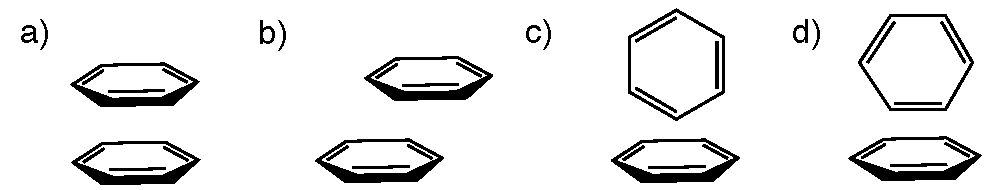
\includegraphics[width=0.7\linewidth]{1Intro/Stacking.pdf}
  \caption[Stacking motifs of benzene]{Packing motifs of benzene molecules: a) face-centred, b) displaced, c) Perpendicular T-shaped, d) Perpendicular Y-shaped. Adapted from ref.~\citenum{Martinez2012}.}
  \label{figure: Benzene_Stacking}
\end{figure}

This intermolecular interaction is detrimental to solid-state fluorescence, and yet is a direct consequence of the design requirements of the chromophore. In biosensing applications, researchers resorted to using dilute solutions with reduced sensitivity because of \ac{ACQ}.\cite{Thomas2007,Kwok2015} In the solid state, for instance in thin films for optoelectronics, the \ac{ACQ} effect means that solution screening for viable candidates is rendered meaningless by the differing luminescent properties of the final material compared to the molecule. Strategies to circumvent \ac{ACQ} have seen varying success, for example through the inclusion of bulky substituents, polar groups, and promotion of hydrogen bonding.\cite{Hong2009,Zhang2013,Mei2014,Mei2015} However, synthetic modification can in turn effect the chromophore's electronic structure and its excited state properties, thus commencing tedious a trail-and-error optimisation process. Attempts to physically block aggregation by encapsulating in surfactants or polymer matrices require extensive engineering and can reduce charge transport.\cite{Hong2009,Chen2000,Lee2013} 

The deleterious effects of \ac{ACQ} cannot be underestimated and pose a significant problem for organic luminescent applications. In the next section of this chapter, we shall look in more detail of the photophysics of molecular aggregates, within the context of Kasha's exciton theory.
%%%%%%%%%%%%%%%%%%%%%%%%%%%%%%
\subsection{Photophysics of Molecular Aggregates}\label{section: lom intermolecular-interactions}
Intermolecular interactions become photophysically important in the solid state due to the dense packing of molecular units. This effect is typically framed in Kasha's two state exciton theory.\cite{Gierschner2009,Gierschner2013,Gierschner2013a,Hestand2017,Shi2017} The exciton is typically defined as a deloclised excited state, where the excited electron and hole remain in close proximity. The Coulomb interaction between the transition dipoles of the monomers in a dimer results in an energy shift in the absorption spectrum, and has underpinned exciton theory since its inception in the 1960s.\cite{Kasha1965a} When two monomers stack ``side-by-side", the Coulombic electronic coupling is positive, a blue-shifted absorption spectrum is witnessed (relative to the isolated monomer) and radiative decay is reduced. This stacking motif is denoted a H-aggregate. Conversely, in J-aggreagtes, dimers align ``head-to-tail", and a red-shifted absorption is witnessed with an increased radiative decay. These extreme cases have helped interpret the supermolecular photophenomena in molecular aggregates.

When the intermolecular distance is large enough to prevent orbital overlap, the exciton can be considered as the interaction of the wavefunction of one monomer ($\ket{1}$) with the wavefunction of the second monomer ($\ket{2}$). In the excited state, the  wavefunctions interact to form a delocalised exciton (a Frenkel exciton), the Hamiltonian $H$ of which is given
\begin{equation}
H=\hbar\omega + \mathrm{\hbar{}D} + J_{0}\{\ket{1}\bra{2}+\ket{2}\bra{1}\}.
\end{equation}
The first term is the energy gap between S\textsubscript{0} and S\textsubscript{1},  $\hbar{}D$ is the shift of the S\textsubscript{1} state in going from the vacuum to the crystal, and $J_{0}$ is the Coulombic coupling.\cite{Spano} The exciton for a multisite system can be described using periodic boundary conditions to produce a wavelike function $k$. For the two site system, $\ket{k}$ is\cite{Hestand2018}
\begin{equation}
\ket{k}=\frac{1}{\sqrt{2}}[e^{ik}\ket{1}+  e^{i2k}\ket{2}]\qquad\quad k=0,\pm{\pi}.
\end{equation}
For the allowed values of $k$, the transition energy $E_k$ for state $k$ is an eigenvalue of $H$, and has the form
\begin{equation}
\mathrm{E}_{k}=\hbar\omega + \mathrm{\hbar{}D} +J_{0}\cos{k}.
\end{equation}
For the two site system, this results in two exciton states in the Frenkel Hamiltonian, as depicted in Figure \ref{figure: H_J_Aggregates}. The Coulomb coupling $J_{0}$ represents the interaction energy due to exchange of excitation energy between $\ket{1}$ and $\ket{2}$, the sign of which dictates whether the symmetric superposition is the upper or lower state. When the coupling is positive, the symmetric state is the upper state, as in the H-aggregate, and the transition dipoles are reinforced resulting in absorption is blue-shifted compared to the gas-phase monomer. Since emission usually takes place from the lower state, where transition dipoles moments cancel, the state is nonradiative and fluorescence is quenched. When the coupling is negative, the symmetric state is lowered and emission is symmetry allowed.\cite{Hestand2017}
\begin{figure}[H]
\centering
  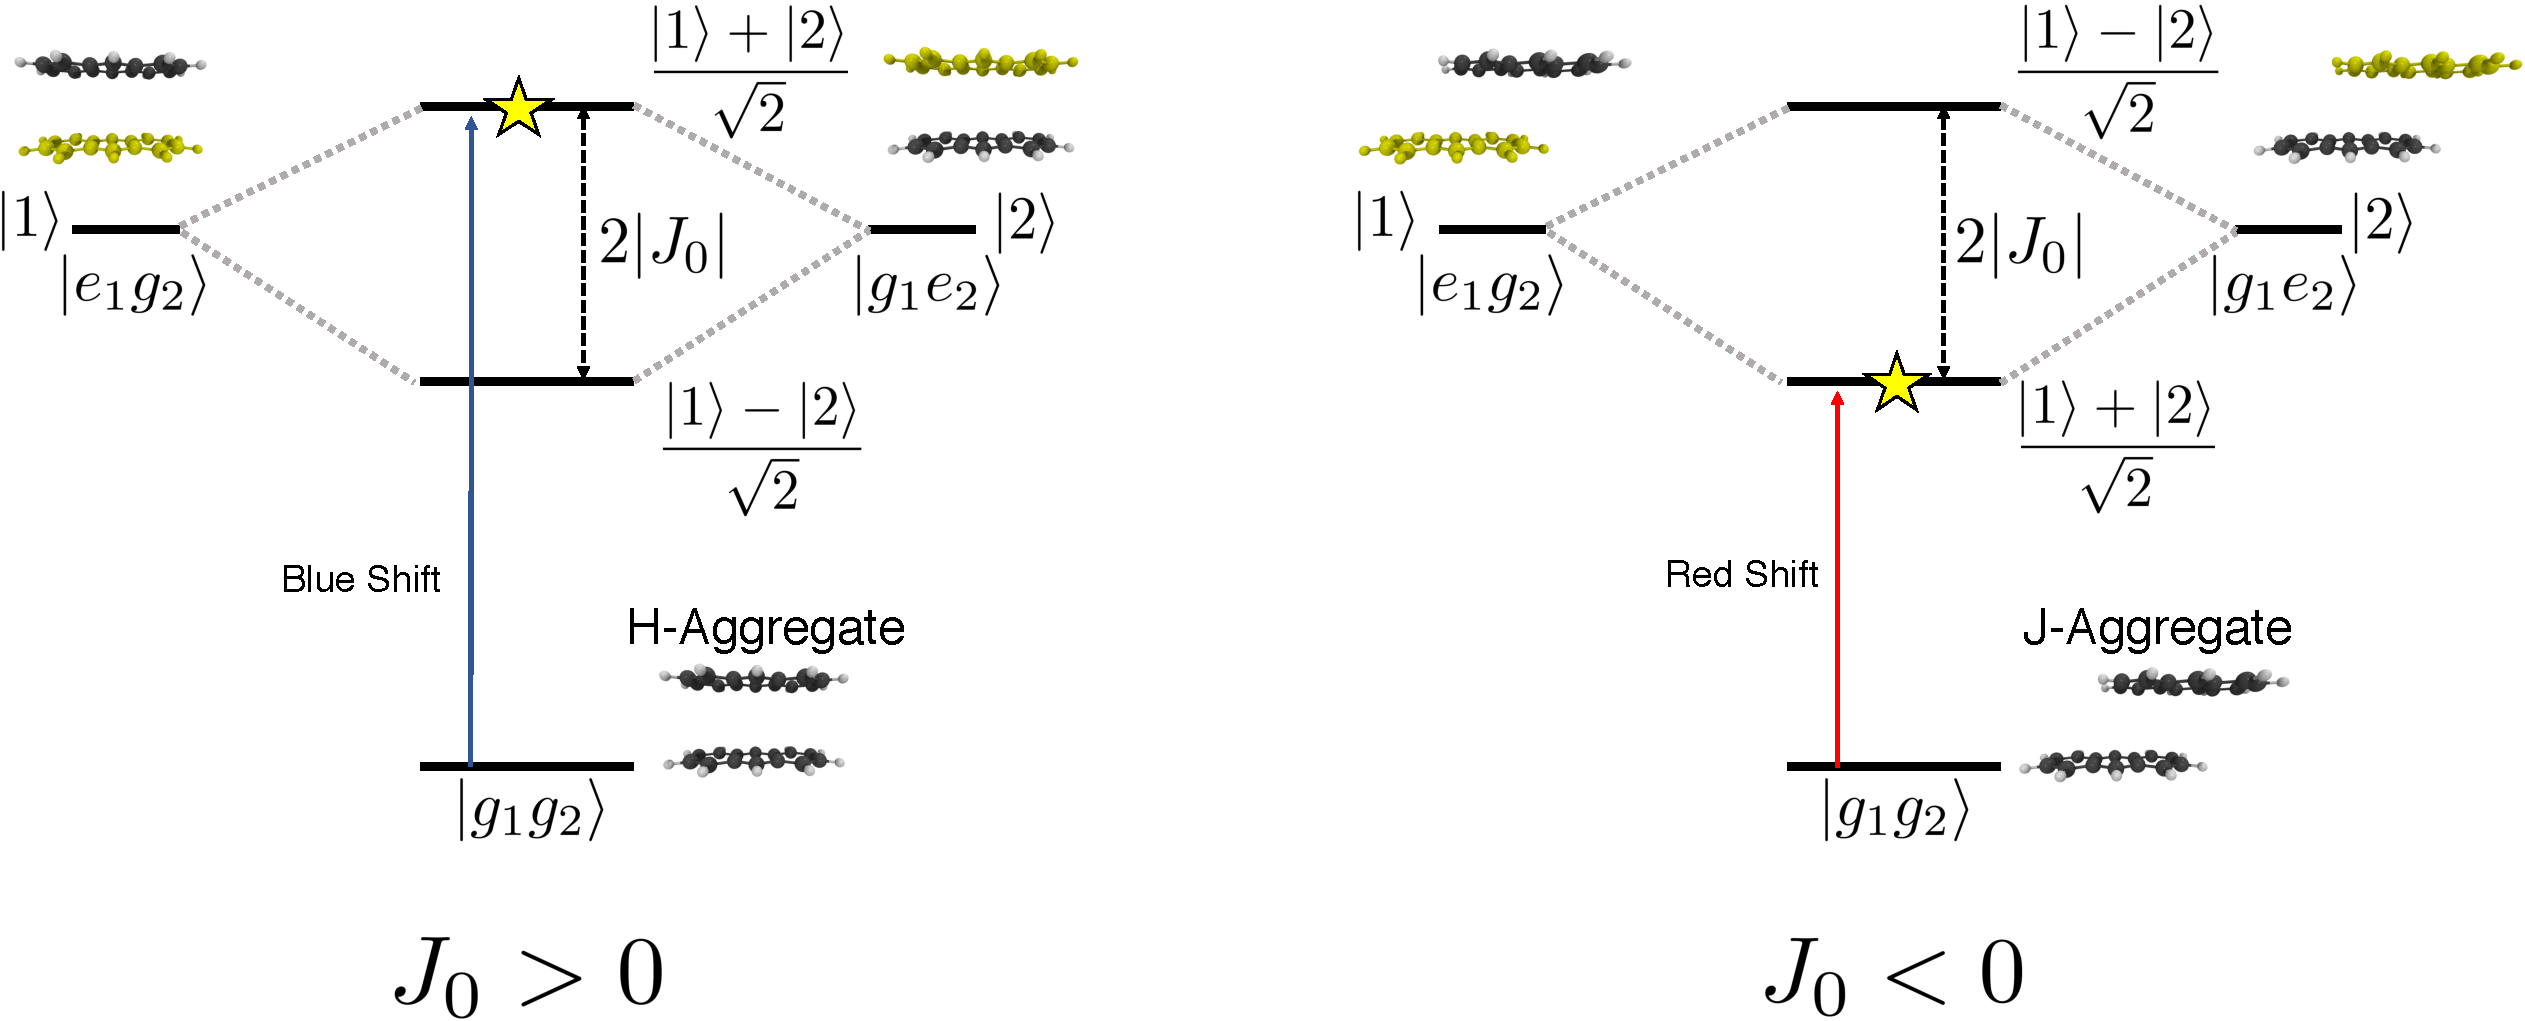
\includegraphics[width=\linewidth]{1Intro/H_J_aggregates.pdf}
  \caption[Exciton energy level diagram for H- and J-aggregates]{Energy level diagram for a H-aggregate (left) and J-aggregate (right) of naphthalene. For the H-aggrgate, the Coulombic coupling $J_{0}$ is positive, raising the energy of the symmetric state resulting in blue-shifted absorption with respect to the monomer state. Emission from the lower state is forbidden, and thus quenched. In the J-aggregate, the negative Coulombic coupling results in red-shifted absorption and allowed emission. The bright excitonic state, the symmetric superposition of the monomer wavefunctions, is indicated with a star.}
  \label{figure: H_J_Aggregates}
\end{figure}
\begin{comment}
\begin{equation}
\ket{g_{1}g_{2}}
\end{equation}
\begin{equation}
\ket{e_{1}g_{2}}
\end{equation}
\begin{equation}
\ket{g_{1}e_{2}}
\end{equation}
\begin{equation}
J_{0}>0
\end{equation}
\begin{equation}
J_{0}<0
\end{equation}
\begin{equation}
2|J_{0}|
\end{equation}
\begin{equation}
\frac{\ket{1}+\ket{2}}{\sqrt{2}}
\end{equation}
\begin{equation}
\frac{\ket{1}-\ket{2}}{\sqrt{2}}
\end{equation}
\begin{equation}
\ket{1}
\end{equation}
\begin{equation}
\ket{2}
\end{equation}
\end{comment}
H- and J-aggregates represent the two extreme stacking cases. In Kasha's theory, the coupling $J_{0}$ arises from the interaction of the transition dipole moments, which at its most crude can be treated as the interaction between two point dipoles,
\begin{equation}
    J_{0,Coul}=\frac{\mu^{2}(1-3\cos^{2}\theta)}{4\pi\epsilon{}R^3}
\end{equation}
where $R$ is the intermolecular distance (between the centroids of the monomers), $\theta$ is the angle between  $\bm{\mu}$ (transition dipole vector) and $\bm{R}$, and $\epsilon$ is the optical dielectric constant of the medium. Thus for H-aggregates, when $\theta=90$, the coupling is positive, and is negative in J-aggregates when $\theta$ is close to zero. H-aggregates become J-aggregates at the so-called ``magic angle" of 54.7\textdegree.\cite{Hestand2018}

The crude point-dipole, Coulomb interpretation of the coupling is only valid approximation for homodimers with large intermolecular separation.\cite{Kistler2013} When monomers stack in close proximity ($R\leq4\si{\angstrom}$), wavefunction overlap invokes the possibility of \ac{CT} states, where the electron resides on one site and the hole on another.\cite{Darghouth2018} This creates a short-range coupling factor as well as the long-range Coulomb coupling. The total coupling is the combined short-range \ac{CT} coupling and the Coulomb coupling, leading to complex behaviour which is dependent on the sign of the short- and long-range contributions. For example, the \ac{CT} coupling is highly sensitive to the molecular geometry, where small distortions can change the total coupling value and result in multiple H- to J-aggregate conversions.\cite{Arago2015} The two components of the total coupling has lead to an expanded nomenclature for stacking motifs, where the contribution of both the short and long-range coupling is considered (HH, HJ, JH, JJ). In the JH and HJ, the interference is completely destructive and the total coupling is zero, resulting in an absorption spectrum at the same position as a monomer.\cite{Hestand2017}

Understanding the complex photophenomena of molecular aggregates is important in the development of materials requiring control over the exciton. The existence of exitons and the dynamics in the solid state, opens nonradiative decay channels and often a quenching of fluorescence for typical aromatic motifs. This has hindered the development of solid-state organic lumniscence. However, this changed when the group of Ben Zhong Tang found a system which had its fluorescence switched on, rather than quenched, upon aggregation - launching a new strategy for the design and development of brightly luminescent organic materials. They named the phenomenon  \acf{AIE}. In the next section of this chapter, the roots of \ac{AIE} shall be examined and the technological advances that have arisen from the discovery briefly outlined.

%%%%%%%%%%%%%%%%%%%%%%%%%%%%%%
%%%%%%%%%%%%%%%%%%%%%%%%%%%%%%
\section{Aggregation Induced Emission}\label{section: lom AIE}
%%%%%%%%%%%%%%%%%%%%%%%%%%%%%%
\subsection{Overview}
In 2001, the Tang group at the Hong Kong University of Science and Technology were interested in silole-based polymers for highly emissive thin-films. As was common at the time, fabrication of such materials was challenging due to \ac{ACQ}. Through serendipity during a purification process, they found that a wet spot of 1-methyl-1,2,3,4,5-pentaphenylsilole was almost non-emissive, but brightly fluorescent after solvent evaporation.\cite{Luo2001} The law of aggregation quenching emission had been turned on its head, and the Tang group had observed the exact opposite behaviour, of molecular aggregation inducing light emission. This was almost unheard of for small organic molecules. 

The Tang group used the \ac{AIE} phenomeon to develop a range of chemical sensors, to detect for instance volatile organic compounds, explosives, and pH.\cite{Dong2007,Li2005,Li2009} Such was the magnitude of the \ac{AIE} breakthrough and the mechanistic interpretations provided by the Tang group, many other groups began to explore this exciting new phenomenon for a wide range of applications. In the field of biological probing, \ac{AIE}-active systems can detect important small molecules such as glucose, thiols, and lactic acid.\cite{Wang2014,Yuan2014,Shen2012} Probes have been developed to detect protein fibrillation, which has been linked to Alzheimer's, Parkinson's and type II diabetes.\cite{Hong2012} \ac{AIE} systems have been also used in medical imaging, where fluorescence is an attractive technique due its high resolution, wide applicability, and low cost.\cite{Mei2015} The Tang group have tracked the progress of the field with periodic, in-depth reviews of the vast number of innovations, of which they contribute a significant share.\cite{Hong2009,Wang2010a,Hong2011,Mei2014,Hu2014,Mei2015}
\subsection{Optoelectronic Applications of AIE}
Upon discovery of \ac{AIE}, the potential for the improvement of optoelectronic devices was immediately apparent. In the original publication, the group built a highly emissive blue-emitting electroluminescent device, and optimised the device to 8\% \ac{EQE} in the cyan region, a vast improvement on the previous high of just 1.5\% for an \ac{OLED}. \cite{Luo2001,Chen2002} \ac{EQE} is the product of the electroluminescence efficiency of the emitter (the organic layer in this case) and the external coupling factor, which is a measure of the fraction of light able to escape the \ac{OLED}. Due to electroluminescence efficiency being limited to 25\% for singlet emitters, and the external coupling being limited to around 22\%, it was previously thought that the theoretical maximum \ac{EQE} is 5.5\%. Indeed, such was the remarkable \ac{EQE} measure in this \ac{OLED} that these previously accepted limitations had to be reconsidered.

In follow-up work, a light-blue emitting \ac{OLED} with hexaphenylsilole (Figure \ref{figure: HPS_TPE}) as the emitting layer was fabricated with \ac{EQE} of 7\%.\cite{Chen2003} While the unfavourable spin statistics inhibit efficiency for singlet-emitting \acp{OLED} across the visible spectrum, deep blue emitters are harder still since the large band gap makes charge injection difficult, hindering the development of full colour displays. Non-doped deep blue \acp{OLED} with \ac{EQE} of around 4\% were reached in 2014, with emitters based on triphenylamine and tetraphenylethene (Figure \ref{figure: HPS_TPE}).\cite{Huang2014,Huang2014a} This has recently been increased to 6.5\% using a carbazole-based organic layer, and in 2018 reached 9.4\%.\cite{KumarKonidena2017,Tang2018} This represents a high for non-doped singlet blue emitters. Inclusion of phosphorescent or thermally-activated delayed fluorescent dopants can further increase the quantum efficiency by harvesting triplet states for luminescence.\cite{Zhu2018}

\begin{figure}[H]
\centering
  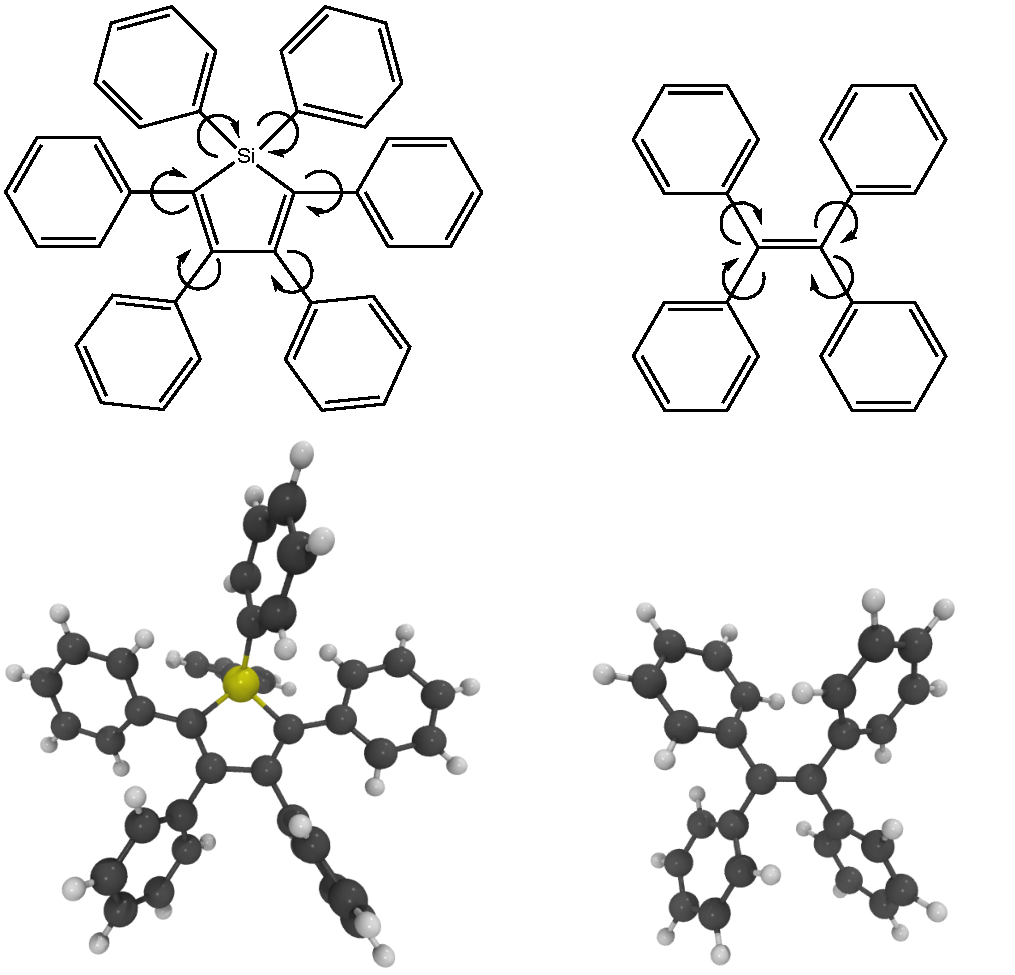
\includegraphics[width=0.7\linewidth]{1Intro/HPS_TPE.pdf}
  \caption[Examples of AIE-active chromophores]{Two dimensional (top) and three dimensional (bottom) structures of two of the ubiquitous AIE-active systems, hexaphenylsilole (HPS, left) and tetraphenylethene (\ac{TPE}, right). AIE occurs through restriction of the rotational motions depicted with arrows.}
  \label{figure: HPS_TPE}
\end{figure}
\subsection{Hypothesised Mechanisms}
Systems exhibiting \ac{AIE} are typically based on a propeller architecture, where a central stator is connected to a number of aromatic rotors via single bonds, as shown in Figure \ref{figure: HPS_TPE}. In the initial analysis of 1-methyl-1,2,3,4,5-pentaphenylsilole, the absorption spectra showed that after the water fraction in an ethanol-water solvent mixture rose above 60\%, the absorption band increased in intensity and moved to longer wavelengths.\cite{Luo2001} On this basis, the \ac{AIE} activity was attributed to the formation of aggregates which forced the molecules into a more planar conformation, thus increasing the conjugation and the absorption. Enough rotation about the sigma bonds was still possible to prevent complete planarity and therefore limiting the stacking and subsequent fluorescence quenching. 

A few months later, the group showed the \ac{AIE} effect for four more silole systems, followed by an extensive study of ten phenylsiloles.\cite{Tang2001,Chen2003} Crucially, in this later work the crystal structure of the siloles showed that the conformation remains twisted in the solid state.\cite{Chen2003} Large torsional angles exist between the phenyl groups and the central silole moiety, on account of the steric repulsion between the six phenyl groups. The lack of space between the phenyl blades, and their angular orientations, prevents intermolecular stacking which give rise to aggregation caused quenching. Therefore the planarisation hypothesis was wrong. 

The group investigated other quenching mechanisms, such as \ac{TICT}, where a non-emissive twisted conformer is formed via charge separation in the chromophore. The \ac{TICT} state can be stabilised, and thus favoured, in polar solvents. However, no emission was recorded across a wide range of solvent polarities for the siloles, ruling out \ac{TICT} as the cause for \ac{AIE}. Also, the lack of electron donor and acceptor groups make it highly unlikely that \ac{TICT} could take place in the siloles. In an elegant experiment it was found that the emission increased almost linearly with increasing solvent viscosity, even though no aggregates were formed. In a similar vain, the photoluminescence intensity increased with decreasing temperature, with NMR studies confirming that the intramolecular rotations of the exterior phenyl groups were reduced at lower temperatures. It was concluded the in good solvents, at ambient temperature, the energy consumed by the rotation of the phenyl groups about the single bonds results in the nonradiative decay of the excited state decay. Upon aggregation, the propeller-like shape limits the intermolecular stacking. Strong C-H\textperiodcentered\textperiodcentered\textperiodcentered$\pi$ interactions rigidify the structure, hindering the intramolecular rotation and the excited state decays via fluorescence.\cite{Chen2003}

The \ac{RIR} mechanism allowed the library of \ac{AIE}-active systems to be expanded to other molecules with propeller-shaped structures. Along with the phenylsiloles, \ac{TPE} derivatives (Figure \ref{figure: HPS_TPE}) have driven understanding and technological progress in the field.\cite{Hong2009,Wang2010a,Hong2011,Mei2014,Hu2014,Mei2015} By switching a phenyl group of \ac{TPE} with a traditional \ac{ACQ} molecules, such as triphenylamine or carbazole, the electroluminscence properties of the system are enhanced due to the hole-transport properties of the \ac{ACQ} group.\cite{Chan2014} Conversely, \ac{ACQ} cores can be made to undergo \ac{AIE} by the attachment of \ac{TPE}.\cite{Yuan2010a}

Dissipation of the excited state can occur through means other than rotation. A bent, $\pi$-surface system of benzenes fused with cyclooctatetraenes undergoes \ac{AIE} but without any rotable units.\cite{Nishiuchi2013} In solution, ring inversions dissipate the excited state and there is almost no emission. Single crystals show emission in the blue region, since the bent structure prevents facial stacking and the inversion modes are restricted. Thus \ac{AIE} is achieved through \ac{RIV}. In a similar vain, the \ac{RIV} mechanism can be applied to \ac{TPE} by locking pairs of phenyl groups with eythlene linkers. In 2014, Tang unified the \ac{RIR} and \ac{RIV} interpretations under the \ac{RIM} umbrella.\cite{Leung2014}

The discovery and development of the \ac{AIE} phenomenon has transformed the field of luminescent organic materials. While much of the innovation has been based on the propeller systems, a class of systems based on \ac{ESIPT} have attracted interest in recent years for their favourable photochemical properties. \ac{ESIPT} systems form the basis of the research in this thesis and in the next section the \ac{ESIPT} mechanism shall be introduced, along with the key applications which incorporate \ac{ESIPT}.
%%%%%%%%%%%%%%%%%%%%%%%%%%%%%%
\section{Excited State Intramolecular Proton Transfer}\label{section: lom ESIPT}
%%%%%%%%%%%%%%%%%%%%%%%%%%%%%%
\subsection{Combining AIE with ESIPT}
Tautomerism is a type of isomerism resulting in the transfer of a chemical group (usually a proton) between two sites on a molecule, and the simultaneous switching of a single and double bond. Photo-induced tautomerism, where the transferring group is a proton, is called \acf{ESIPT}. Research into the mechanism and potential applications of ESISPT has been active for more than half a century, since \ac{ESIPT} was first observed in the 1950s in salicylic acid. Photochromic materials harnessing \ac{ESIPT} have garnered much attention due to the wide range of applications and remarkable properties. In particular, it is the unusually large Stokes-shifted emission which makes \ac{ESIPT} so attractive. The separation between the absorption and emission wavelengths can typically exceed 200 nm, reducing self-absorption and increasing the output signal for the desired application. The emission colour can be tuned by the addition of electron donating or withdrawing groups, as well as solvent polarity and viscosity.\cite{Azarias2016,Yushchenko2007} Dual emission from the pre- and post-\ac{ESIPT} forms is also possible. These characteristics, in tandem with \ac{AIE}, have resulted in \ac{ESIPT} chromophores being used for chemical sensing, biological imaging and probing, as well the optoelectronic applications such as optical memory, lasers, and \acp{OLED}.\cite{Hsieh2010,Kwon2011,Zhao2012,Demchenko2013,Padalkar2015,Chen2018}
\begin{figure}[H]
\centering
  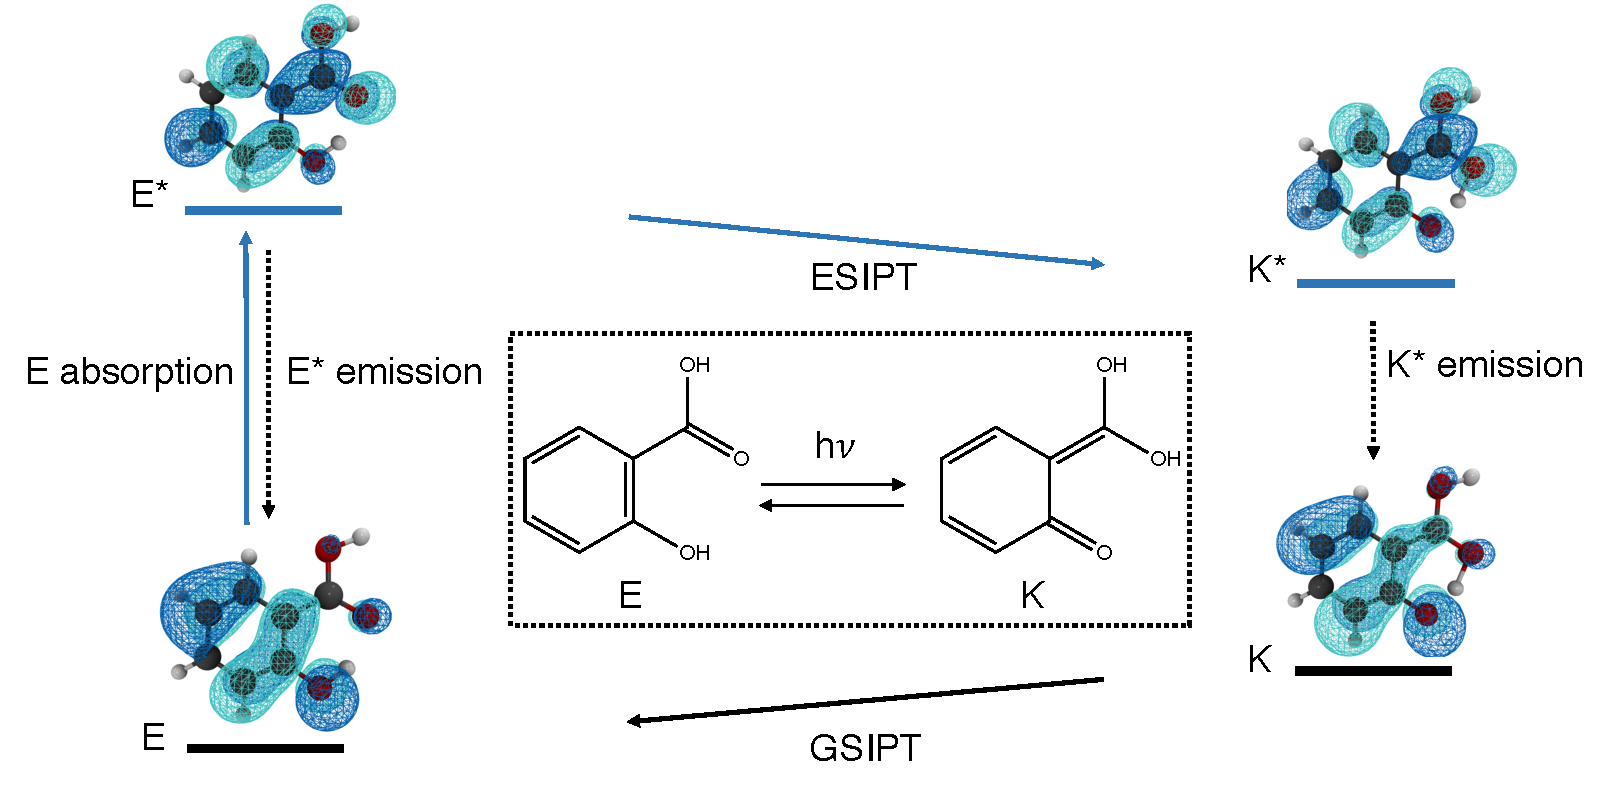
\includegraphics[width=0.95\linewidth]{1Intro/ESIPT.pdf}
  \caption[The four-level photocycle of \ac{ESIPT}]{The four-level photocycle of \ac{ESIPT} for salyclic acid. The HOMO and LUMO orbitals for tautomer are also shown.}
  \label{figure: ESIPT}
\end{figure}
\subsection{The Four-Level Photocycle}
Inherent in all \ac{ESIPT} processes is a fully reversible four-level photocycle, the prerequisite for which is the presence of an intramolecular hydrogen bond. The proton donor can be an amino or hydroxyl group, while the proton acceptor is usually an imine or carbonyl. The four-level photocycle for salicylic acid is depicted in Figure \ref{figure: ESIPT}, along with the main molecular orbitals. The chromophore in the ground state (S\textsubscript{0}) is in the enol form (E), mediating hydrogen bond formation between the carbonyl oxygen and the hydroxyl proton. Upon electronic excitation, the excited state (\Estar, S\textsubscript{1}) the geometry remains unchanged but electronic redistribution acidifies the hydroxyl and increases the basicity of the carbonyl group, as a result of the population of the $\pi^\ast$ orbital on the carbonyl oxygen. In the excited state, the keto form (\Kstar) is more stable due to the redistributed electron density, and the proton migrates from the hydroxyl oxygen to the carbonyl oxygen. Depending on the system, fluorescence can occur from both the excited enol form (\Estar) and the excited keto form (\Kstar), although due to the ultrafast nature of the proton transfer the major emitting species is the keto tautomer.\cite{Zhao2012} For most \ac{ESIPT} processes containing strong hydrogen bonds, proton transfer is near barrierless and  occurs on a femtosecond time scale.\cite{Padalkar2015} The rate of the proton transfer and emission wavelength are highly sensitive to the surrounding medium and the presence of electron donor/acceptor moieties.\cite{Demchenko2013,Lin2017a,Li2017c} After fluorescence, the ground state keto form (K) is populated and the four level photocycle (E$\rightarrow$E$^{\ast}$$\rightarrow$K$^{\ast}$$\rightarrow$K) is completed. The initial geometry is restored through \ac{GSIPT}, although other photoproducts can be formed, for instance through cis-trans isomerisation or intersystem crossing.\cite{Al-Soufi1990}

\ac{AIE} in \ac{ESIPT} chromophores can be more complex than in non-polar propeller systems. The presence of hydrogen bonding sites enables the formation of intermolecular hydrogen bonds with solvent molecules, weakening the intramolecular bond and hindering \ac{ESIPT}.\cite{Cheng2015f} Kasha showed that the ratio of fluorescence intensity between \Estar and \Kstar dramatically changes based upon the solvent polarity.\cite{Kasha1986} In 3-hydroxyflavanone, the \Kstar fluorescence band is suppressed and the \Estar band increases in intensity with polar solvents. In strongly basic solvents, intermolecular proton transfer can occur between the chromophore and solvent, blocking access to the \Kstar state\cite{Laurent2014}. As touched upon earlier, the presence of donor acceptor groups opens the possibility of deactivation through \acf{TICT}. In solvent, the \ac{TICT} state is populated after proton transfer and lead to nonradiative decay. In a similar vain to \ac{RIR}, aggregation frustrates the torsional mode, preventing the \ac{TICT} from forming, and opens the radiative decay channel.\cite{Park2017,Wu2015a}
\subsection{Exploiting ESIPT and AIE for Applications}
The most investigated class of \ac{ESIPT} molecules are based on benzothiazole dyes, particularly \ac{HBT}.\cite{Padalkar2015,Kwon2011} The groups of Li and Liu investigated the effect of solvent for a range of \ac{HBT} derivatives, finding that increasing polarity impedes the proton transfer reaction and diminishes fluorescence. This is compounded by highly polar, protic solvents, where the hydroxyl proton can dissociate to form the phenolic anion. The proton transfer is highly sensitive to the solvent polarity, which is highly useful for sensing and probing applications.\cite{Wang2009,Cheng2015f} A \ac{HBT} analogue has been developed for ratiometric probing for hydrogen peroxide in living cells, where the \ac{ESIPT}-active fluorophore is produced by oxidative hydrolysis.\cite{Tang2018a} \ac{HBT}-based systems are also applicable for pH sensing, ion detection, biothol probing, and intracellular imaging.\cite{Kachwal2018,Kachwal2018,Liu2018}

Substitution of electron donor and acceptor groups onto \ac{ESIPT} cores can alter the proton transfer rate and stability of the enol and keto conformers on the excited state potential energy surface. In an extensive theoretical study, Jacquemin and co-workers investigated how different substitution patterns affect the emission from enol and keto states for a range of benzothiazoles.\cite{Azarias2016} They found that dual emission from both E$^*$ and K$^*$ is only possible in a small energy window for the compounds tested, and that the K$^*$ minimum can be favoured more drastically by dependent on the heteroatom in the core. The strongest substituent effects are seen with electron donor groups, such as methoxy, which stabilise the E$^*$ state. The K$^*$ state can be favoured by electron withdrawing groups in particular positions. Crucially, the effects of combining substituent groups is complex and depend on the specific \ac{ESIPT} core and substituent combination. The easily purturbed electronic structure of these systems make design from first principles extremely challenging.

\ac{ESIPT} cores are excellent candidates for optoelectronic applications on account of minimised self-absorption. However, the environment sensitivity which makes them so suitable for probing can be harmful to device stability.\cite{Kwon2011} Through chemical modifications, the Park group have fabricated stable \ac{OLED} devices with a range of emission frequencies.\cite{Park2008,Park2009,Kim2011} Introduction of carbazole gave access to blue K$^*$ emission, while \ac{EQE} values of 14\% have been reached by incorporating triplet harvesting via thermally activated delayed fluorescence with \ac{ESIPT}.\cite{Park2008,Mamada2017} Emission from both E$^*$ and K$^*$ enables white-light emission in devices, a highly attractive property due to the rarity of single molecule fluorophores with wide emission bands.\cite{Tang2011,Yao2011,Zhang2016b,Serdiuk2017}

The population inversion afforded by the \Kstar form makes \ac{ESIPT} systems attractive for laser applications.\cite{Fang2014,Gierschner2016} Additionally the large Stokes shift limits reabsorption and increases the optical gain.\cite{Kwon2011} In the 1980s, the principle of using \ac{ESIPT} for lasing applications was established by Kasha and co-workers for 3-hydroxyflavone, where the ultrafast proton transfer and double-well excited state potential energy surface lead to efficient population inversion.\cite{Khan1983,Chou1984} Since then, the structural diversity of \ac{ESIPT} systems have produced lasers with emission in the green, orange, and cyan regions.\cite{Sakai2016,Chen2016,Park2012,Park2008} Recently, an imidazole-based system with amplified spontaneous emission properties was developed with deep blue emission.\cite{Park2017} The restriction of the \ac{TICT} state in the crystalline form results in quantum yield of fluorescence of 67\%, producing an intense and narrow blue band for emission. 
\subsection{Emission Characteristics of 2'-hydroxychalcones}
Developing efficient fluorophore emission at the extremes of the visible spectrum is notoriously difficult. Whilst much attention has been paid to the blue region, the red and \ac{NIR} region is also hugely challenging in the solid state. The first system to exhibit solid state lasing properties in the \ac{NIR} region was reported in 2015.\cite{Cheng2015} The compounds were based on \ac{HC} skeletons and displayed \ac{ESIPT}. Interestingly, solid state fluorescence is only witnessed in some analogues, with substituent position and crystal packing modes determining the quantum yield of fluorescence. The question of whether electronic effects or the crystal structure determined the fluorescence activity was not fully resolved. Fluorene-containing derivatives with laser properties were published soon after.\cite{Cheng2016} In the same year, the same group published another breakthrough in solid state lasing, with structures based on  \ac{HP}.\cite{Tang2016} These compounds are similar to the \acp{HC}, but contain only one aromatic ring. Solid state fluorescence in single-benzene emitters is a rarity due to low melting points, but these systems showed extremely high fluorescence activity, surpassing the parent \ac{HC} systems.

For the \ac{HC} and \ac{HP} systems, the crystal packing, absorption and emission wavelength, andcrucially the QE, are all dependent on the choice of substituent and number of aromatic rings. How these factors interplay is not well understood. To fully understand the photophysical properties of these systems, intricate knowledge of the electronic, molecular picture must be combined with the intermolecular interactions inherent in the crystal as a whole. Theoretical methods can help elucidate this picture and offer insight into the working mechanisms behind \ac{AIE} for these \ac{ESIPT} systems, and how to maximise the quantum yield of fluorescence. This is the primary aim of the work in this thesis, with \ac{HC} and \ac{HP} families used as exemplars. In the next section, the properties of \ac{HC} and \ac{HP} shall be examined, with main focus on the parent \ac{HC} compounds. 
%%%%%%%%%%%%%%%%%%%%%%%%%%%%%%
\section{Emitters based on 2'-hydroxychalcones}\label{section: lom HC}
%%%%%%%%%%%%%%%%%%%%%%%%%%%%%%
\subsection{Spectroscopic Investigations}
Research into \acp{HC}, and chalcones in general, has traditionally revolved around their metabolite character, since they are in vivo precursors for a variety of flavones, flavonols, isoflavones, anthocyanidins, and other synthetic antioxidants.\cite{Singh2014} \acp{HC} also show \ac{ESIPT} fluorescence in the \ac{NIR} region upon aggregation. The \ac{ESIPT} process in \ac{HC} was first proven by Chou et al. in 1992.\cite{Chou1992} With an absorption band at 354 nm, and emission at 635 nm, the authors concluded that tautomerisation occurs upon absorption and that the keto S\textsubscript{1} state was responsible for emission. Cis-trans isomerism about the central double bond followed by molecular oxygen incorporation produces the flavanoid studied by Kasha, 3-hydroxyflavone. Previous studies had investigated this cyclisation mechanism, where it was initially thought cyclisation occurred through cis-trans isomerisation without proton transfer.\cite{Stermitz1975,Matsushima1985} It was later found that this isomerism could be hindered by solvent viscosity.\cite{Tokumura1998} Later, Arai and coworkers investigated the photochemistry of \textbf{HC} analogues, where they denoted the tautomerisation to be hydrogen atom transfer, rather than proton transfer.\cite{Arai1997,Norikane2002,Norikane2003,Kaneda2003,Kaneda2003a,Kaneda2004,Teshima2009} They mapped the potential energy surfaces using spectroscopic techniques to find that the cis-trans isomerism takes place in the triplet state, and only after hydrogen atom transfer. Most pertinent was their study of the effect of substituent on fluorescence in 2009.\cite{Teshima2009}  Studying systems solvated in benzene, they found that the addition of a methoxy substituent in the \textit{para} position of the phenol ring increased the quantum yield of red fluorescence by at least ten times, which the authors attribute to a combination of electronic and steric effects. The methoxy group stabilises the S\textsubscript{1} state through electron donation to the carbonyl \pipistar orbital whilst its size hinders the intramolecular modes. 
%%%%%%
\subsection{Cyrstalline Emission Properties}
%%%%%%
More recently, \textbf{HC} compounds have been developed for sensing and imaging applications. In 2014, the Tang group (of \ac{AIE} fame), developed a ratiometric fluorescent probe for sensing alkaline phosphatase based on 2'-hydroxychalcone.\cite{Song2014} Alkaline phosphotase is a dephosphorylating  enzyme, high concentration of which acts as a biomarker for diseases such as hepatitis, prostate cancer, and bone issues. By replacing the hydroxyl group of \textbf{HC} with a phosphoric acid group, the emission is yellow in aqueous conditions. In the presence of alkalane phosphotase, the cleave of phosphate and yields 2'-hydroxychalcone, which undergoes \ac{ESIPT} and emits in the red region. Another probe was developed to detect cysteine, again through the activation of \ac{ESIPT}.\cite{Li2017a} The \ac{AIE}/\ac{ESIPT} principle was applied using \textbf{HC} to develop a technique to detect latent fingerprints, for example in crime scenes.\cite{Jin2015} A fingerprint contains a high level of sebum, and when this is rinsed a \textbf{HC} solution, the \textbf{HC} molecules preferentially adhere to the fatty acid residues in the fingerprint, where they aggregate. When light is shone on the fingerprint, \ac{ESIPT} occurs and red fluoresence is produced, lighting up the fingerprint region against the dark backdrop of the substrate. 

In 2015, Zhang et al. synthesised a range of crystalline \textbf{HC} systems with different substitution patterns.\cite{Cheng2015} They found the identity and the position of the substituent to be critical in the quantum yield of the crystals. This is summarised in Figure \ref{figure: HC_experimental}. When substituents are \textit{meta} to  the hydroxyl group (compounds \textbf{1}-\textbf{3}) in the phenol ring, deep red fluorescence is observed, but only when in crystalline form. The solutions are almost non-emissive. Interestingly, under frozen conditions the solutions still only weakly fluoresce, indicating that restriction of intramolecular rotation is not the key factor in the \ac{AIE} for these molecules. When the same substituents are in \textit{para} position (compounds \textbf{4},\textbf{5}), neither the crystals nor the solutions are emissive. 
\begin{figure}[H]
\centering
  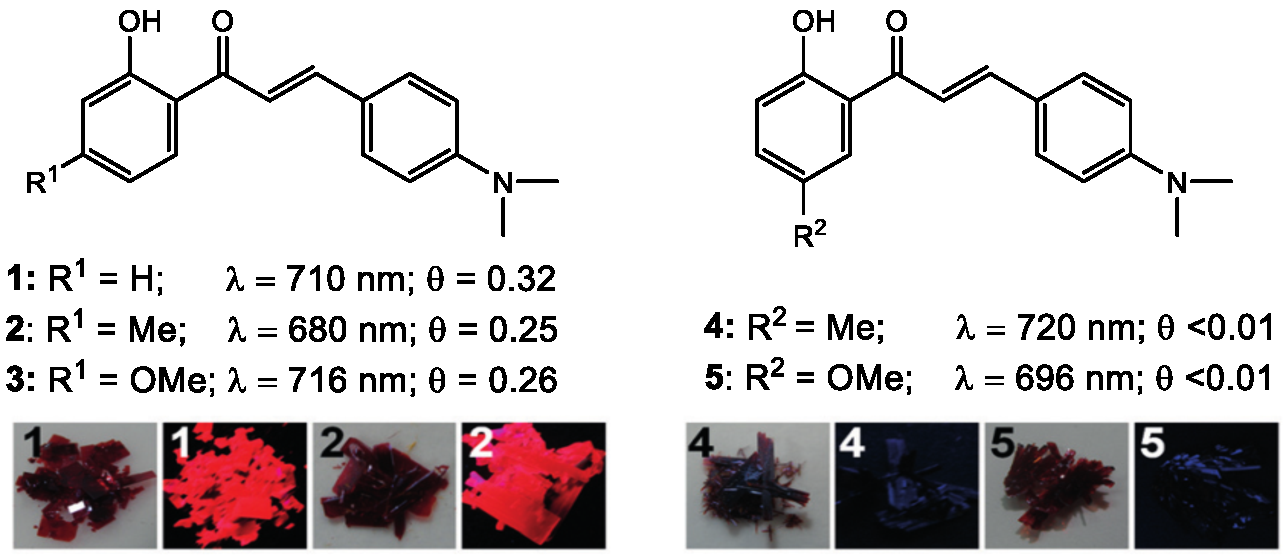
\includegraphics[width=0.95\linewidth]{1Intro/HC_experimental.pdf}
  \caption[Emission behaviour of crystalline 2'-hydroxychalcone derivatives]{Compounds \textbf{1}-\textbf{5} synethised by Zhang and coworkers. \textbf{1}-\textbf{} show high quantum yield, but \textbf{4}\&\textbf{5} are almost non-emissive. Absorbance maxima ($\lambda$) and quantum yields of fluorescence ($\theta$) are given, along with pictures of the dark and bright crystals for \textbf{1},\textbf{2},\textbf{4}, and \textbf{5}. Figure adapted from ref.~\citenum{Cheng2015} with permission of Wiley-VCH.}
  \label{figure: HC_experimental}
\end{figure}
These puzzling characteristics are attributed to both the planarity of the individual molecules and the packing in the crystal, as shown in Figure \ref{figure: HC_stacking}   Molecules \textbf{1}-\textbf{3} are almost completely planar and the strong intramolecular H-bonds, of length 1.753-1.780 \si{\angstrom}, increase the rigidity and planarity of the system. In the crystal, the molecules adopt an edge-to-face, herringbone packing mode preventing intermolecular $\pi$-interactions between the aromatic rings and enabling fluorescence from the keto S\textsubscript{1} state. For compound \textbf{4}, where a methyl substituent is \textit{para} to the hydroxyl, a similar edge-to-face packing mode is present. However, the molecule has a larger dihedral angle than \textbf{1}-\textbf{3}, which the authors attribute as the reason for the weak fluorescence. For \textbf{5}, the molecule is planar but the packing is face-to-face with aromatic stacking interactions. In the discussion, it is asserted that \textbf{5} is therefore non-emissive in the solid state due to excimer formation and non-radiative decay. The authors also hypothesise that the edge-face packed crystal of compound \textbf{4} shows minimal fluorescence because the molecule is not planar, despite other edge-face packed molecules brightly fluorescing, while the planar molecule does not emit because it is packed face to face.
\begin{figure}[H]
\centering
  \includegraphics[width=0.95\linewidth]{1Intro/HC_stacking}
  \caption[Crystal structures of 2'-hydroxychalcone derivatives]{The conformation of monomers \textbf{1},\textbf{4}, and \textbf{5}, along with their crystal structure. Crystal structures obtained from CCDC database codes from ref.~\citenum{Cheng2015}.}
  \label{figure: HC_stacking}
\end{figure}
It is with these hypotheses that this thesis begins. The first fundamental question is why do none of the five compounds fluoresce in good solvent? Secondly, in the solid state, why do only compounds \textbf{1}-\textbf{3} exhibit \ac{AIE}. Is this a substituent effect, as a result of the position of the methyl and methoxy groups, or is it due to the molecular packing mode, or is it a combination of both? Quantum chemical methods can identify the nonradiative decay channels in both dispersed and aggregated states, and therefore can elucidate the discrete electronic and intermolecular factors. In answering these questions, we can build understanding of how structure-property relationships operate in the \ac{AIE}/\ac{ESIPT} space. 
%%%%%%%%%%%%%%%%%%%%%%%%%%%%%%
\section{Structure of thesis}\label{section: lom outline}
%%%%%%%%%%%%%%%%%%%%%%%%%%%%%%




\chapter{Chemistry on a Computer}
\newcommand{\schro}{Schr\"{o}dinger}
\label{chapter:theory}
\section{Quantum Mechanics and Chemistry}\label{section: QM}
\subsection{Overview}\label{section: QM_overview}
The development of quantum mechanics in the early 20th century armed scientists with the tools to calculate the microscopic properties of matter. In chemistry, the postulates of quantum mechanics can be applied to calculate relative energies of molecules, molecular geometries, ratios of products of chemical reactions, transition states, spectra, and any other phenomenon of interest. However, whilst in principle any property can be calculated exactly by the \schro{} equation, the analytical solution is only obtainable for systems with one electron. For systems larger than this, and therefore anything of observable chemical relevance, the computational expense on even modern computer architecture is intractable. 

To overcome this, a number of approximations are used field of computational chemistry. In general, as the number of atoms one wants to model increases, qualitative nature of the result also increases. Computational chemistry methods can generally be split into the types of approximations made and the number of atoms the method wishes to treat. In biophysical process and the modelling of proteins on the scale of tens of thousands of atoms, quantum mechanics is ignored completely. Forcefields are used to calculate the energy corresponding to a set of atomic coordinates in what are known as the \ac{MM} class of methods. The interactions between atoms are defined by analytical potentials, such as for bond stretches, bends, and angles, and are parameterised for different types of molecules using more accurate methods. This procedure is time-consuming and makes the forcefield specific to the systems it was fitted to, but enables computationally facile access to molecular geometries and properties of large systems.

At the other end of the scale, for systems of typically less than 500-1000 atoms, the electronic structure is included through wavefunction or \ac{DFT} techniques. For the applications involved in this thesis, involving photoinduced phenomena, the activity of the electrons is paramount, and as such it is these methods which are utilised herein. In the next sections, the importance of the \schro{} equation shall be established, which along with the Born-Oppenheimer approximation enables the calculation of electronic properties through the simplest wavefunction method, the \ac{HF} method. Methods to improve the \ac{HF} approximation are then introduced, followed by the paradigm shift offered by \ac{DFT}. This chapter mainly focuses on methods to obtain ground state properties, whilst in Chapter X excited state methods shall be discussed. 
%%%%%%%%%%%%%%
%%%%%%%%%%%%%%
\subsection{The \schro{} Equation}\label{section: QM_schrodinger}
%%%%%%%%%%%%%%
%%%%%%%%%%%%%%
The wavefunction $\Psi$ contains all the information about the quantum state of the system at a position and time. As Newton's second law ($\bm{\mathrm{F}}=m\bm{\mathrm{a}}$) gives a classical particle's position and moment at each time period, thus describing it's classical state, so the time-dependent \schro{} equation does for wavefunction, and has the general form
\begin{equation}\label{equation: td-schro}
    i\hbar{}\frac{\partial \Psi(\bm{R},\bm{r},t)}{\partial t}=\hat{H}\Psi(\bm{R},\bm{r},t)
\end{equation}
where $\hbar=\frac{h}{2\pi}$ and $\hat{H}$ is the Hamiltonian operator for electrons at $\bm{r}$ and nuclei at $\bm{R}$. Separating the spatial part from the temporal part of differential time-dependent \schro{} equation yields the time-dependent version of the \schro{} equation, which using the bra-ket notation of Dirac is
\begin{equation}\label{equation: ti-schro}
   \hat{H}\ket{\Psi}=E\ket{\Psi}.
\end{equation}
This is an eigenvalue equation, where the Hamiltonian operator acts on the wavefunction to give the energy $E$ of the system. For a system of $N$ electrons and $M$ nuclei, the Hamiltonian calculates the kinetic ($T$) and potential ($V$) energy contributions of the electrons and nuclie towards the total energy of the system,
\begin{equation}\label{equation: H-simple}
\hat{H}=\hat{T}_{e}+\hat{T}_{n}+\hat{V}_{n-e}+\hat{V}_{e-e}+\hat{V}_{n-n}
\end{equation}
\begin{equation}\label{equation: H}
   \hat{H}=\underbrace{-\sum_{i=1}^{N}\frac{1}{2}\nabla_{i}^2 - \sum_{A=1}^{M}\frac{1}{2M_{A}}\nabla_{A}^2}_\text{kinetic terms}-\underbrace{\sum_{i=1}^{N}\sum_{A=1}^{M}\frac{Z_{A}}{r_{iA}}+\sum_{i=1}^{N}\sum_{j>{i}}^{N}\frac{1}{r_{ij}}+\sum_{A=1}^{M}\sum_{B>{A}}^{M}\frac{Z_{A}Z_{B}}{R_{AB}}}_\text{electrostatic terms}
\end{equation}
where $i$ and $j$ are electrons and $A$ and $B$ are nuclei. The first two terms are the operators for the kinetic energy of the electrons and the nuclei, where the Laplacian operator $\nabla^{2}$ is the second derivative of position. The next three terms are the electrostatic operators, summing the Coulomb interactions in the system;  the attractive interaction between electrons and the nuclei (of charge $Z$); the repulsive interaction between electrons; and the repulsive interaction between nuclei. Atomic units are used throughout, such that the electronic charge and mass are neglected. The $R$ and $r$ terms in the electrostatic parts denote the distance between nuclei and electrons.
%To calculate the energy $E$ , however, an eigenfunction for Equation \ref{equation: ti-schro}is required, corresponding to a wavefunction describing the electronic state.\cite{aszabo82:qchem}

In the hydrogen atom, the $\hat{V}_{e-e}$ and $\hat{V}_{n-n}$ can be neglected since there is only one proton and one electron, and the exact solution for the energy can be calculated since the wavefunction can be constructed analytically. However, for larger systems with many electrons and nuclei, Equation \ref{equation: ti-schro} cannot be solved. As such, a number of approximations must be made. The most fundamental of these is Born-Oppenheimer approximation, which shall be introduced in the next section.
%%%%%%%%%%%%%%
%%%%%%%%%%%%%%
\subsection{The Born-Oppenheimer Approximation}\label{section: QM_bornoppenheimer}
%%%%%%%%%%%%%%
%%%%%%%%%%%%%%
Separation of variables is a key concept in quantum chemistry, where a complex problem is broken down into constituent parts. This method is used to simplify the solving of Equation \ref{equation: ti-schro} by separating the electronic terms from the nuclear terms. This is rooted in the fact that the nuclei are vastly heavier than electrons, and so it can be approximated that the nuclei are static with respect to the electrons. Equation \ref{equation: ti-schro} is solved, then, in two steps. First, the electronic structure is solved with ``clamped" nuclei, resulting in an electronic energy which is a parametric function of the nuclear coordinates. By concentrating on just the electronic terms, the \textit{electronic} Hamiltonian $\hat{H}_{e}$ becomes
\begin{equation}\label{equation: Hel}
     \hat{H}_{e}=\underbrace{-\sum_{i=1}^{N}\frac{1}{2}\nabla_{i}^2}_\text{kinetic term}-\underbrace{\sum_{i=1}^{N}\sum_{A=1}^{M}\frac{Z_{A}}{r_{iA}}+\sum_{i=1}^{N}\sum_{j>{i}}^{N}\frac{1}{r_{ij}}}_\text{electrostatic terms}.
\end{equation}
and the electronic \schro{} equation is then
\begin{equation}\label{equation: ti-schro-el}
   \hat{H}_{e}\ket{\Phi}=E_{e}\ket{\Phi}
\end{equation}
The total wavefunction $\Psi$ is reconstructed from the the combination of the electronic functions for each state $I$ and the corresponding nuclear wavefunction $\Theta_{I}$
\begin{equation}
    \Psi(\bm{R},\bm{r})=\sum_{I}\Theta_{I}\Phi_{I}.
\end{equation}

When the nuclei are stationary, their kinetic energy is zero and the complete Hamliltonian is just the electronic Hamiltonian. For vibrating molecules, Equation \ref{equation: ti-schro-el} is solved at the required nuclear configuration, for electronic state $I$, and the time-evolution of the nuclear wavefunctions is
\begin{equation}\label{equation: nucwavefunctions}
    i\hbar{}\frac{\partial{}\Theta_{I}}{\partial{}t}=[\hat{T_{n}}+E_{I}]\Theta_{I}\underbrace{-\sum_{I}\hat{\Lambda}_{JI}\Theta_{I}}_\text{Nonadiabtic couplings}
\end{equation} 
%%%%%%%%%%%%COMMENT
\begin{comment}
\begin{equation}
    \sum_{A}\frac{1}{2M_{A}}\sum_{J\neq{}I}\hat{\Lambda}_{JI}\Theta_{I}=[\hat{T_{n}}+E_{I}(\bm{R})-E]\Theta_{I}
\end{equation} 
\end{comment}
%%%%%%%%%%%%COMMENT
where the energy of $E_{I}$ is the expectation value of the electronic Hamiltonian ($\bra{\Phi_{I}}\hat{H_e}\ket{\Phi_{I}}$). The highlighted \textit{nonadiabtic coupling} operator $\hat{\Lambda}_{JI}$ couples electronic state $I$ with electronic state $J$. In the adiabatic Born-Oppenheimer approximation, this coupling is completely neglected and the time-evolution of the nuclei becomes
\begin{equation}\label{equation: BO}
    i\hbar{}\frac{\partial{}\Theta_{I}}{\partial{}t}=[\hat{T_{n}}+E_{I}]\Theta_{I}
\end{equation} 
The nuclear motion is thus determined by the electronic energy of uncoupled \textit{adiabatic} states, and the nuclei move on the \ac{PES} of state $I$. $\hat{\Lambda}_{JI}$ contains the \textit{nonadiabatic} couplings, which become important when electronic states converge in energy. This shall be discussed in Section \ref{section: photo_conicals}

The Born-Oppenheimer approximation helps divide the problem into electronic and nuclear parts. However, solving the electronic problem exactly for many electron systems is impossible. In the next section, methods to solve the electronic problem are introduced, starting with the \acf{HF} method. The \ac{HF} method is the fundamental quantum chemical approach to solve the many electron problem.
%%%%%%%%%%%%%%
%%%%%%%%%%%%%%
\section{Quantum Chemical Methods}\label{section: methods}
\subsection{The Hartee-Fock Method}\label{section: methods_HF}
%%%%%%%%%%%%%%
%%%%%%%%%%%%%%
In the \ac{HF} method, the intractable $N$-electron wavefunction $\Phi$ is simplified to be a product of $N$, one-electron wavefunctions $\chi$,
\begin{equation}
\ket{\Phi}=\ket{\chi_{1}\chi_{2}...\chi_{i}..\chi_{N}}.
\end{equation}
 where $\chi$ are spin orbitals of each electron in the system. The spin orbitals consist of a spatial functional and a spin function, an infinite number of which will provide an exact solution. However, in practical terms a basis set is supplied, where molecular orbitals are made of (typically) linear combination of Gaussian functions, representing atomic orbitals. Whilst Gaussian functions themselves do not reflect the correct atomic orbital behaviour seen in Slater-type functions, the combination of multiple Gaussians can recover the radial behaviour along with the many numerical advantages. 
 
 From the Pauli exclusion principle, no two electrons may share exactly the same four quantum numbers (i.e occupy the same spatial and spin orbital). Since electrons are fermions, the electronic wavefunction is \textit{antisymmetric}, meaning that a change in the orbital must result in the wavefunction changing sign. This is enforced using Slater Determinants. This is most easily seen for a two-electron system for electrons at positions $\bm{x}_{1}$ and $\bm{x}_{2}$, where orbital $\chi_{1}$ contains electron at $\bm{x}_1$ and orbital $\chi_{2}$ contains electron at $\bm{x}_2$, with a normalisation factor of $N^{-\frac{1}{2}}$
\begin{equation}
\begin{split}
\Phi(\bm{x}_{1},\bm{x}_{2})&=\frac{1}{\sqrt{2}}\{\chi_{1}(\bm{x}_{1})\chi_{2}(\bm{x}_{2})-\chi_{1}(\bm{x}_{2})\chi_{2}(\bm{x}_{1})\}\\
&=\frac{1}{\sqrt{2}}
\begin{vmatrix}
\chi_{1}(\bm{x}_{1})&\chi_{2}(\bm{x}_{1})\\
\chi_{1}(\bm{x}_{2})&\chi_{2}(\bm{x}_{2})
\end{vmatrix}
\end{split}
\end{equation}
where by taking the determinant, the antisymmetry is ensured since exchanging the electrons changes the sign of the determinant. In the determinant, the rows consist of the electrons while the columns contain the orbitals. In the \ac{HF} method, the wavefunction is approximated by a single Slater Determinant, and therefore \ac{HF} is known as a single-determinant, or single-reference, method.  As well as ensuring antisymmetry, the Slater determinant wavefunction also introduces exchange, where the motion of two electrons with the same spin is correlated. This means that the probability of finding one electron at a certain position is dependent on the position of an electron of the same spin at another position, and the probability of finding the two electrons at the \textit{same} point in space in zero. This is not true for electrons of opposing spin, and thus antiparallel spins are uncorrelated in the \ac{HF} method.

The variational principle states that the true ground state wavefunction will always be less than or equal to a trial wavefunction, meaning that the guessed spin orbitals will never undershoot the true energy. As such, 
\ac{HF} is a purely iterative method where the energy is computed for a set of trial spin orbitals, the spin orbitals are altered, and the energy is guessed again. This is repeated until convergence. 

To calculate the ``best" set of orbitals, the interactions in the electronic Hamiltonian are split into one-electron and two electron terms. The one electron terms are collected by the core Hamiltonian operator $\hat{h}_{i}$, involving the kinetic energy of the electrons and the electron-nuclei interactions,
\begin{equation}
    \hat{h}_{i}=-\frac{1}{2}\nabla_{i}^{2}-\sum_{A=1}^{M}\frac{Z_{A}}{r_{iA}}.
\end{equation}
The antisymmetric nature of the Slater determinent results in two operators for the electron-electron interaction, a Coulomb operator $\hat{J}_{ij}$ and an exchange operator $K_{ij}$, which act on orbital $\chi_{i}$ to determine the effect of the remaining orbitals,
\begin{equation}
    \hat{J}_{ij}\chi_{i}=\chi_{i}\int{\frac{\chi^{\ast}_{j}\chi_{j}}{r_{ij}}d\bm{x}_{2}}
\end{equation}
\begin{equation}
    \hat{K}_{ij}\chi_{i}=\chi_{j}\int{\frac{\chi^{\ast}_{j}\chi_{i}}{r_{ij}}d\bm{x}_{2}}.
\end{equation}
The Coulomb operator determines the Coulomb potential felt by electron $i$ in orbital $\chi_{i}$ from electron $j$ in orbital $\chi_{j}$. This is done by \textit{averaging} the interaction over all of the spatial coordinates of electron $j$. As such, $J_{ij}$ represents the average, or \textit{mean-field}, local potential felt by electron $i$. For this reason, the \ac{HF} method is often called a mean-field approach. The exchange operator $K_{ij}$ is a result of the antisymmetric Slater determinant, and is a quantum mechanical artefact of the fact that electrons are by nature  indistinguishable, and the exact labelling ($i$,$j$) has no physical meaning. 

The one-electron and two-electron operators are collected by the Fock operator $\hat{F}$, such that
\begin{equation}
    \hat{F}=\hat{h_{i}}+\sum_{j\neq{}i}^{\frac{N}{2}}{[\hat{J_{ij}}-\hat{K_{ij}}]}
\end{equation}
The two electron terms run over only half of the electrons ($\frac{N}{2}$) to ensure interactions are not double counted, while the condition of $j\neq{}i$ means that an electron cannot interact with itself. 

The Fock operator allows Equation \ref{equation: ti-schro} to be solved in the \ac{HF} method through,
\begin{equation}\label{equation: Fock-operator}
    \hat{F}\ket{\Phi}=E\ket{\Phi}
\end{equation}
an eigenvalue equation solved by altering the linear combination of basis functions until energy convergence is reached. In practice, for a closed shell system, the molecular orbital $\chi_{i}$ consists of a linear combination of $K$ atomic basis functions,
\begin{equation}\label{equation: expansion}
    \chi_{i}=\sum_{\mu=1}^{K}C_{ui}\phi_{\mu}\qquad\quad{}i=1,2,..,K
\end{equation}
The Roothaan equations are then used to solve Equation \ref{equation: Fock-operator} in matrix form,
\begin{equation}
    \bm{FC}={\bm{SC\epsilon}}
\end{equation}
where $\bm{F}$ is the Fock matrix containing the elements from the Fock operator, $\bm{C}$ contains the expansion coefficients from Equation \ref{equation: expansion} and $\bm{S}$ is the overlap matrix containing the overlaps of atomic orbitals ($\bra{\phi_{i}}\ket{\phi_{j}}$). By diagonalising the Fock matrix, $\epsilon$ is a diagonal matrix containing the orbital energies. \ac{HF} is commonly named the \ac{SCF} approximation, since the Roothaan equations are solved until self-consistency is reached.


The \ac{HF} method is a powerful approach to solving the electronic part of the \schro{} equation. However, it has several severe drawbacks which hinder its application and have resulted in more sophisticated methods being developed to address the shortcomings within. The most serious of these for ground state, closed-shell systems is the correlation problem. While electrons of parallel spin have the required exchange correlation, the Coulomb correlation is completely neglected since each electron sees only an average field of the other electrons. In reality, the motion of one electron is dependent on the motion of each of the other electrons (Figure \ref{figure: mean-field}), and the energy of the system in \ac{HF} is overestimated in respect to the true energy. A number of methods to overcome the lack of correlation have been developed, which use the \ac{HF} method as a starting point before calculating the electron correlation. These are called post-Hartree-Fock methods, and those most relevant to the work in this thesis are discussed in the next section.
\begin{figure}[H]
\centering
  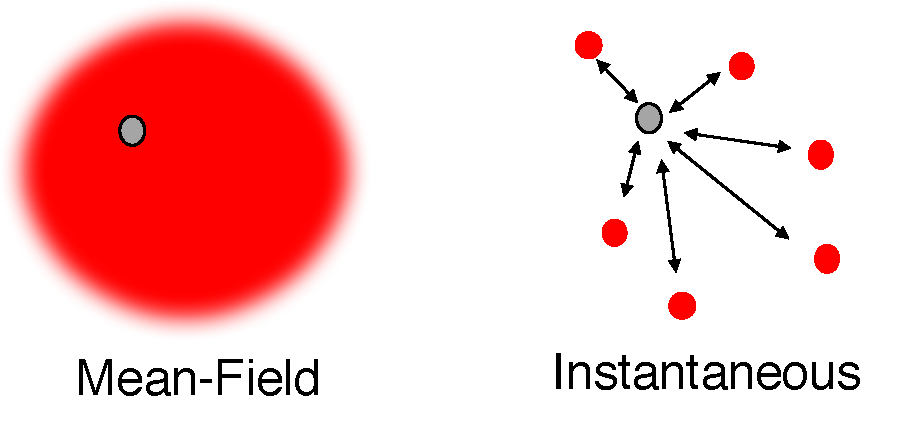
\includegraphics[width=0.4\linewidth]{2Theory/Mean_Field.pdf}
  \caption[Schematic of the mean-field approximation]{Depiction of the mean field electron interaction, where the electron of interest interactions with an average potential, rather than individually with each other electron.}
  \label{figure: mean-field}
\end{figure}
%%%%%%%%%%%%%%
%%%%%%%%%%%%%%
\subsection{Post-Hartre-Fock Methods}\label{section: methods_postHF}
%%%%%%%%%%%%%%
%%%%%%%%%%%%%%
\subsubsection{M{\o}ller-Plesset Perturbation Theory}
%%%%%%%%%%%%%%
Electron correlation energy can be added to the \ac{HF} energy by way of an external perturbative correction. In perturbation theory, the total Hamiltonian is divided into the zeroth-order part $\hat{H}_{0}$, which is the \ac{HF} Hamiltonian, and a perturbation $\hat{V}$, such that the eigenvalue equation becomes
\begin{equation}\label{equation: PT}
    \hat{H}\ket{\Phi_{i}}=(\hat{H}_{0}+\hat{V})\ket{\Phi_{i}}=\epsilon_{i}\ket{\Phi_{i}}.
\end{equation}
The eigenvalues and eigenfunctions of $\hat{H}_{0}$ are varied so that they become closer to the total Hamiltonian $\hat{H}$, which would then contain electronic correlation. This is done by the ordering factor $\lambda$, such that
\begin{equation}
    \hat{H}=\hat{H}_{0}+\lambda\hat{V}
\end{equation}
The true eigenvalues and eigenfunctions are expanded in a Taylor series in $\lambda$ up to $n$th order,
\begin{equation}\label{equation: MP2_energies}
    \epsilon_{i}=E_{i}^{(0)}+\lambda{}E_{i}^{(1)}+\lambda^{2}E_{i}^{(2)}+\lambda^{3}E_{i}^{(3)}+..+\lambda^{n}E_{i}^{(n)}
\end{equation}
\begin{equation}\label{equation: MP2_functions}
    \ket{\Phi_{i}}=\ket{\Phi_{i}^{(0)}}+\lambda{}\ket{\Phi_{i}^{(1)}}+\lambda^{2}\ket{\Phi_{i}^{(2)}}+\lambda^{3}\ket{\Phi_{i}^{(3)}}+..+\lambda^{n}\ket{\Phi_{i}^{(n)}}
\end{equation}
After inserting Equations \ref{equation: MP2_energies} and \ref{equation: MP2_functions} into Equation \ref{equation: PT} and collecting terms by order, the general expression for the total energy is
\begin{equation}
E_{i}=E_{i}^{(0)}+\sum_{n=1}^{n}\bra{\Phi_{i}^{(0)}}\hat{V}\ket{\Phi_{i}^{(n-1)}}
\end{equation}
The perturbation operator $\hat{V}$ introduces the Coulomb repulsion between electrons, which when combined with excited Slater determinants, recovers the \textit{dynamic} correlation energy. In most chemical applications, the method is contracted at second-order, and was initially employed by C. M{\o}ller and M.S. Plesset to obtain the correlation energy, hence the acronym \ac{MP2} is often used.\cite{Moller1934} Since MP is perturbative, the MP-calculated energy can be lower than the true energy, making it a non-variational method.
%%%%%%%%%%%%%%
\subsubsection{Coupled Cluster Theories}
%%%%%%%%%%%%%%
In an alternative approach to perturbation theory, \ac{CC} methods were introduced in the 1960s to account for electron correlation.\cite{Cizek1966,Paldus1972} \ac{CC} theory uses excited determinants by means of a Taylor expansion with an exponential operator
\begin{equation}\label{equation: cc}
    \ket{\Phi_{CC}}=e^{\hat{T}}\ket{\Phi_{0}}
\end{equation}
where $\ket{\Phi_{0}}$ is the \ac{HF} wavefunction and $\hat{T}$ is the cluster operator. The cluster operator produces a sum of excitation operators up to the truncation level $n$
\begin{equation}\label{equation: T}
    \hat{T}=\hat{T}^{(1)}+\hat{T}^{(2)}\hat{T}^{(3)}+..+\hat{T}^{(n)}
\end{equation}
where $N$ is the excitation number. So, $\hat{T}^{(1)}$, includes all single excitations and $\hat{T}^{(2)}$ includes all double excitations, \textit{etc}. For the first order, the contribution of all single excited determinants is 
\begin{equation}
    \hat{T}^{(1)}\ket{\Phi_{0}}=\sum_{i}^{occ}\sum_{a}^{vir}t_{i}^{a}\phi_{i}^{a}
\end{equation}
where $\phi_{i}^{a}$ is the excitation of an electron from occupied orbital $\phi_{i}$ to virtual orbital $\phi_{a}$, and $t_{i}^{a}$ is the amplitude given to this excitation. Substituting \ref{equation: T} into \ref{equation: cc}, and truncating at $n=2$, yields the coupled cluster wavefunction
\begin{equation}\label{equation: CCwavefunctioncomplete}
\ket{\Phi_{CC}}=e^{\hat{T}}\ket{\Phi_{0}}=\big[1+\hat{T}^{(1)}+(\hat{T}^{(2)}+\frac{\hat{T}^{2(1)}}{2})\big]\Phi_{0}
\end{equation}
As for perturbation theory, \ac{CC} theory is usually referred to by the trunctation level, for example CCSD refers to coupled cluster with single and double excitations. CCSD scales at $N^{6}$, adding considerable expense to the \ac{HF} method, which scales at $N^{4}$.

%%%%%%%%%%%%%%
\subsection{Multireference Methods}\label{section: methods_multiconf}
%%%%%%%%%%%%%%
The methods described so far use \ac{HF} as a starting point and are thus built on a single-reference wavefunction. For a closed-shell system of an even number of electrons, orbitals are all doubly occupied. However, in many chemical processes, the electronic structure will deviate from this description and the wavefunction will not be dominated by one single electronic configuration, for example in bond dissociation, excited state processes, or when metallic elements are introduced. To describe these scenarios, the ground state wavefunction must incorporate other relevant electronic configurations, where more than one Slater determinant is used in the ground state wavefunction. These are termed multireference or multiconfigurational methods, and the multireference wavefunction is expressed as
\begin{equation}
    \ket{\Psi}=\sum_{m}c_{m}\ket{m}
\end{equation}
where $\ket{m}$ is the configuration state function containing optimized molecular orbitals and $c_{m}$ is the expansion coefficient for the state. In multireference methods, the molecular orbitals are divided into subspaces, where the active space contains the oribitals from which the important configurations are taken. In the configuration interaction method, the active space contains all of the molecular orbitals, with all excitations between the orbitals are considered, and thus all possible configurations are used in the wavefunction. This recovers the exact wavefunction, but is prohibitivaly expensive such is the vast number of possible determinants, although these can be truncated to include only single excited states. More common is to use an active space containing occupied and virtual orbitals selected for their relevance for the problem in hand, and to only include excitations from within the $m$ active orbitals for $n$  electrons. This is called the \ac{CAS} method, which when used in combination with \ac{HF} for the remaining core orbitals (outwith the active space), is denoted \ac{CAS}\ac{SCF}.\cite{Roos1980} Due to the factorial scaling with the number of active orbitals, further space decomposition methods have been introduced through \ac{RAS}, where only certain excitations are allowed. Furthermore, using a state-averaging procedure can optimize the configuration state-functions for multiple states, to describe regions of strong electronic mixing. With these methods, the key parameter is often the choice of the active space - which orbitals to include, how many of them, and how many corresponding electrons. This is not a black-box procedure and will vary depending on the system of interest, the phenomena being modelled, and the computational resources available.\cite{Lischka2018} Recently, algorithms for automatic active-space selection procedures have been proposed.\cite{Stein2016,Bao2018}

Electron correlation can be divided into dynamic and static contributions. By incorporating the multireference character of the wavefunction, \textit{static} correlation is recovered in solving the \schro{} equation. The dynamical part is added on top of a reference wavefunction in the form of excitations, typically through perturbation theory as discussed in \ref{section: methods_postHF}. As such, most of the total correlation can be recovered by combining a multireference wavefunction with perturbation theory. This can produce accurate ground and excited state properties for chemical systems, although with rather large computational expense.\cite{Ramos-Cordoba2017,Stein2016a} A favoured approach is to combine \ac{CAS}\ac{SCF} with a \ac{PT2} calculation (\ac{CAS}\ac{PT2}), providing an effective protocol to calculate excited states. 
\subsection{Density Functional Theory}\label{section: theory_dft}
%%%%%%%%%%%%%%
The methods introduced thus far access chemical properties through some approximation of the wavefunction. An alternative approach is to disregard the wavefunction altogether and instead use the electron density to calculate microscopic properties of matter. This replaces the 3$N$ (+spin) variable of wavefunction methods by just 3 (+spin) spatial variables, allowing significant speed-up in \ac{DFT}. In 1964, Pierre Hohenberg and Walter Kohn proved a unique 1:1 correspondence exists between the ground state energy and the ground state density, and that all ground properties of a given $N$-electron system can be calculated from the ground state electron density ($\rho$).\cite{Kohn1964} The energy is thus a \textit{functional} (function of a function) of the electron density produced by a wavefunction,
\begin{equation}
    E[\rho]=\bra{\Psi[\rho]}\hat{T}+\hat{V}\ket{\Psi[\rho]}
\end{equation}
and, like in \ac{HF}, obeys the variational principle.

\ac{DFT} is a mathematically exact formulation. However, the exact form of the functional relating the density to the energy is unknown. In 1965, Kohn and Sham developed a self-consistent approach to attain an approximation of the energy functional in equations that are ``analogous to the conventional Hartree and Hartree-Fock equations, and, although they also include correlation effects, they are no more difficult to solve."\cite{Kohn1965} In the Kohn-Sham system, a non-interacting system is set up to mimic the real interacting electron density. As in \ac{HF} where one-electron wavefunctions construct the N-electron wavefunction, so do single particle orbitals (Kohn-Sham orbitals $\phi$) construct the electron density,
\begin{equation}
    \rho=\sum_{j=1}^{N}|\psi_{j}|^{2}.
\end{equation}
The Kohn-Sham expression for the energy functional is written in terms of the kinetic and electrostatic interactions,
\begin{equation}
    E[\rho]=T_{e}[\rho]+E_{n-e}[\rho]+E_{e-e}[\rho].
\end{equation}
The most straightforward term to evaluate is the nuclear-electron interaction, which can be expressed as an electrostatic potential $V_{n}$ from the nuclei acting on the electronic density, 
\begin{equation}
    V_{ne}[\rho]=\int{V_{n}(\bm{r})\rho(\bm{r})\mathrm{d}\bm{r}}.
\end{equation}
The electron-electron interaction can be separated into a classical, Coulomb-type expression and the quantum mechanical \ac{XC} part
\begin{equation}
    E_{ee}[\rho]=\frac{1}{2}\underbrace{\int{}\frac{1}{r_{e_{1}e_{2}}}\rho(\bm{r}_{e_{1}})\rho(\bm{r}_{e_{2}})\mathrm{d}\bm{r}_{e_{1}}\mathrm{d}\bm{r}_{e_{2}}}_\text{Classical}+\underbrace{\vphantom{ \left(\frac{a^{0.3}}{b}\right) }E_{ee}^{XC}[\rho]}_\text{Exchange-Correlation}
\end{equation}
The kinetic energy of the interacting system is replaced by the kinetic energy of the non-interacting system, with the correction incorporated in to the \ac{XC} functional. It is the \ac{XC} functional which contains the crux of the problem in \ac{DFT}, since the exact form is unknown. It must be approximated. Much of \ac{DFT} development is focused on developing more accurate functionals to better describe specific chemical problems.

The first approximation to the functional is the \ac{LDA}. The LDA was originally proposed by Kohn and Sham in 1965 and depends only on the density at the coordinate in question. LDA approximates the molecular \ac{XC} energy by the \ac{XC} energy of a uniform electron gas. The \ac{XC} energy at a point in the molecule is then compared to a homogeneous electron gas with that density, for which the exchange can be solved analytically and the correlation is approximated through, for example, Monte-Carlo simulation.\cite{Ullrich2012} LDA works surprisingly well in structure prediction, given that the UEG has a uniform density whereas in reality the density varies with position in molecular systems. To incorporate the change of electron density with position, the \ac{GGA} functions include the density gradient, offering improved total energies, energy barriers, and geometries. Of the \ac{GGA} functionals, the PBE functional has become one of the most used in quantum chemistry.\cite{Perdew1996}

Hybrid functionals improve upon the \ac{GGA}s by including a percentage of \ac{HF} exchange energy. The \ac{XC} energy is expressed as a linear combination of the \ac{DFT} derived \ac{XC} and the \ac{HF} exchange energy. The hybrid version of PBE, PBE0, incorporates exact exchange via
\begin{equation}
    E_{XC}^{PBE0}=\alpha{}E_{X}^{HF}+(1-\alpha{})E_{X}^{PBE}+E_{C}^{PBE}.
\end{equation}


One of the key errors in Kohn-Sham \ac{DFT}, using the types of functionals introduced thus far, is the self-interaction error. In \ac{HF}, the electron-electron interaction of the Hamiltonian ensures that an electron will interact with all the other electrons in the system but itself. In \ac{DFT}, each electron interacts with the entire electron density and thus with itself. If 100\% exact exchange is used this error is exactly cancelled. However, since this is not present in \ac{LDA}s or \ac{GGA}s, the \ac{XC}-potential does not show the correct asymptotic behaviour, and is only partially remedied by the small percentage of \ac{HF} exchange in hybrids. At large interelectronic distances, the self-interaction results in incorrect long-range asymptotic behaviour, where the \ac{XC} potential falls off more rapidly than 1/$R$.

To remedy this, a class of functionals called \acp{RSH} has been developed. The exchange is split into short- and long-range parts, where the short-range exchange will typically be represented by a local or semi-local functional, while the long range exchange is treated by \ac{HF} exchange. The distance at which the behaviour changes is determined by the range-separation parameter. Therefore, the long-range behaviour can be corrected due to having exact exchange. Whilst hybrid functionals are the most widely used in present day computational chemistry, it is certainly not a ``one size fits all" situation, since different functionals are developed to meet certain requirements, with development being ``property-driven" as much as rooted in theory. In particular, for dealing with excited states in \ac{TDDFT}, hybrid functionals have known and systamic failings, which the \ac{RSH} functionals aim to address. This shall be discussed in the next section, where the theory and techniques for modelling excited states are introduced.
%%%%%%%%%%%%%%%%%%%%%%%%%
%%%%%%%%%%%%%%%%%%%%%%%%%
\section{Modelling Electronically Excited States}\label{section: Photo}
%%%%%%%%%%%%%%%%%%%%%%%%%
%%%%%%%%%%%%%%%%%%%%%%%%%
\subsection{Overview}\label{section: photo_overview}
Thus far the methods introduced generally address thermal chemical processes, i.e those which occur in the electronic ground state. Modelling electronically excited states is a considerably more complex task, in terms of both the number of possible reaction paths and the methods needed to describe them. Some of these are illustrated in Figure \ref{figure: Jablonski}. The \acf{PES}, briefly introduced in Section \ref{section: QM_bornoppenheimer}, is absolutely central in understanding excited-state processes. It is through probing the \ac{PES} that feasible pathways, and thus chemical mechanisms, are elucidated and physical observable are rationalised theoretically.

\begin{figure}[H]
\centering
  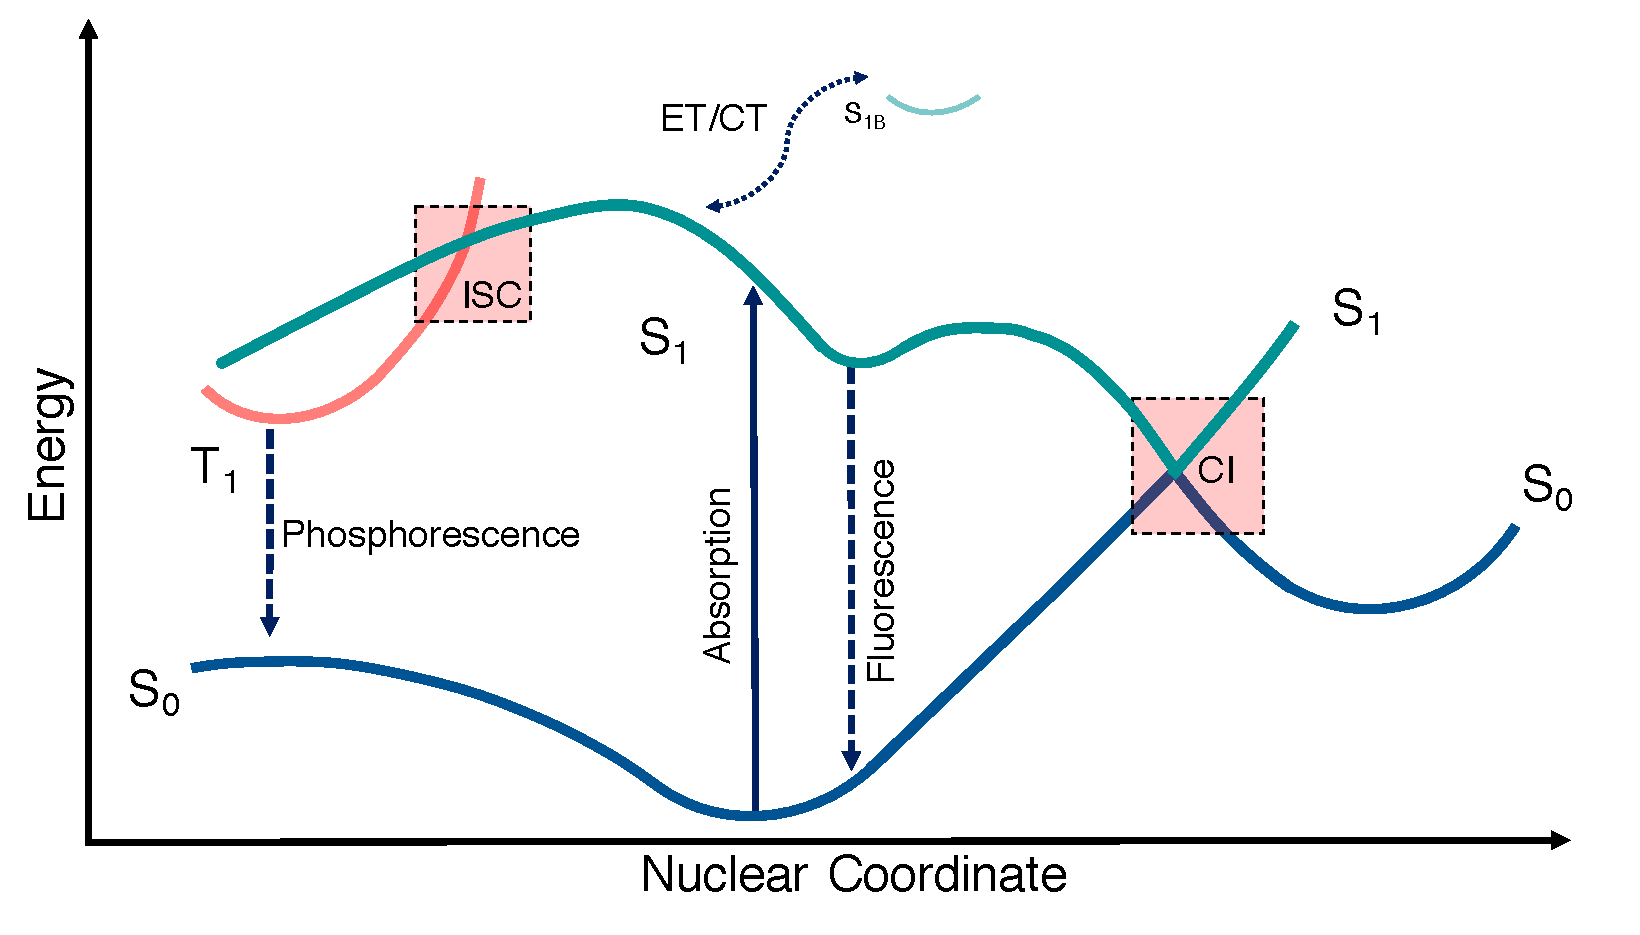
\includegraphics[width=0.8\linewidth]{2Theory/Jablonski.pdf}
  \caption{Competing relaxation pathways after electronic excitation to the first excited singlet state (S\textsubscript{1}. Nonradiative decay channels through conical intersections (CI), energy transfer (ET) and charge transfer (CT) to other molecules, compete with fluorescence. Alternatively, intersystem crossing (ISC) can occur, followed by phosphorescence.}
  \label{figure: Jablonski}
\end{figure}

Electronic excitation, induced by irradiation from the \ac{UV} or visible range, will normally occur at the thermal equilibrium geometry in the ground state. Absorption of a photon will place the system in an electronically excited state. According to the \ac{FC} Principle, the nuclei will undergo negligible change upon change in electronic state. This region of the \ac{PES} is called the \ac{FC} region, or point, and the electronic excitation is considered to be vertical (directly to the point of the upper \ac{PES} vertically above the ground state). From here, a multitude of relaxation processes are possible with vastly different timescales. The fastest process is typically relaxation to lowest vibrational state, occurring in femtoseconds, followed by fluorescence. At the other end of the scale, if there is significant spin-orbit coupling, crossing to a triplet state through \ac{ISC} followed by phosphorescence can take milliseconds. 

Calculating the relative energies of these relaxation pathways is a challenging task for a number of reasons. Firstly, whilst Figure \ref{figure: Jablonski} is a one-dimensional cut of a specific nuclear coordinate, the true \ac{PES} is a 3$N$-6 (3$N$-5 for a linear molecule) hypersurface of nuclear degrees of freedom. As such the full surface cannot feasibly be sampled for large molecules, and specific areas or modes are initally chosen. Secondly, the same ground state methods introduced in Section \ref{section: methods} must be tweaked or expanded upon to incorporate excited states. Thirdly, and perhaps most importantly, in certain regions of the \ac{PES} the fundamental principle of quantum chemical methods, the Born-Oppenheimer approximation, breaks down altogether. Such regions occur when two electronic states become close in energy, as highlighted in red in Figure \ref{figure: Jablonski}. In this region, the electronic states become directly coupled with the nuclear motion, breaking the Born-Oppenheimer approximation. These ``funnel" regions, or conical intersections, are crucial in modelling nonradiatve decay.

This section is organised as follows. Firstly, the importance of conical intersection will be discussed. Following, we will examine how excited-state mechanisms can be probed through nonadiabatic dynamics simulations. Finally, methods to perform these calculations, such as \acf{TDDFT}, shall be addressed. 
\subsection{Conical Intersections}\label{section: photo_conicals}
In photochemical processes with well-defined, well-separated electronic states, the adiabatic Born-Oppenheimer approximation is valid (Equation \ref{equation: BO}). That is, the nuclear wavefunction of an electronic state independent from the nuclear wavefunction of another state. However, as shown in Figure \ref{figure: Jablonski}, in photochemical processes there are regions on the energy landscape where electronic states become close in energy. In these regions, small changes in nuclear configuration results in large changes in the electronic wavefunction - hence the separation of nuclear and electronic wavefunctions is no longer valid and the Born-Oppenheimer approximation breaks down. In practice, this means that the nonadiabtic coupling terms become important and can no longer be neglected. The coupling operator $\Lambda$ of Equation \ref{equation: nucwavefunctions} is defined as
\begin{equation}
    \hat{\Lambda}_{IJ}=\frac{1}{2M}(2\bm{F}_{JI}\cdot{}\nabla{}+G_{JI})
\end{equation}
where 
\begin{equation}
    \bm{F}_{JI}=\bra{\Phi_{I}}\nabla{}\ket{\Phi_{J}}
\end{equation}
is the derivative or nonadiabatic coupling vector with respect to position and $G_{JI}$ is the scalar coupling,
\begin{equation}
    G_{JI}=\bra{\Phi_{I}}\nabla{}^{2}\ket{\Phi_{J}}
\end{equation}
and $\nabla$ the first derivative of position. $\bm{F}_{JI}$ is a 3$N$-vector coupling the nuclear motion of electronic state $I$ with state $J$. The total value is given by the scalar product of $\bm{F}$ with the nuclear momentum, and so the size (and thus the probability of a transition) is defined by the size of the coupling as well as the momentum of the nuclei.\cite{Worth2004}. The derivative coupling $\bm{F}_{JI}$ can be expressed in terms of the electronic Hamiltonian $H_{e}$, such that
\begin{equation}\label{equation: NAC_F}
        \bm{F}_{JI}=\frac{\bra{\Phi_{I}}\nabla{}\hat{H}_{e}\ket{\Phi_{J}}}{E_{J}-E_{I}}.
\end{equation}

With large electronic differences ($E_{J}-E_{I}$), the large mass difference between electrons and nuclei make $Lambda$ inconsequentially small. However, as states converge the coupling increases. Only two coordinates can lift complete degeneracy, resulting in the \ac{PES} forming a double-cone structure. Conical intersections thus act as funnels, where the wavepacket can transfer nonradiatively between electronic states in an ultrafast timeframe. The two degrees of freedom define the branching space vectors. The first is the gradient difference vector $\bm{g}$, defining the difference between the gradients of the upper and lower \acp{PES},
\begin{equation}
    \bm{g}_JI=\bra{\Phi_{I}}\nabla{}\hat{H}_{e}\ket{\Phi_{I}}-\bra{\Phi_{J}}\nabla{}\hat{H}_{e}\ket{\Phi_{J}}.
\end{equation}
The second is the nonadiabatic coupling vector $\bm{h}$, defining the direction of strongest coupling between states, which is the numerator of Equation \ref{equation: NAC_F},
\begin{equation}
    \bm{h}_{JI}=\bra{\Phi_{I}}\nabla{}\hat{H}_{e}\ket{\Phi_{J}}.
\end{equation}
The vectors $\bm{g}$ and $\bm{h}$ are orthogonal, defining the plane of the conical intersection. $\bm{g}$ points in the direction of removing the energetic splitting, whilst $\bm{h}$ points towards maximising the nonadiabatic coupling. This is depicted in Figure \ref{figure: Cone} Important to note is that for polyatomic molecules the conical intersection is not an isolated point but multidimensional. Displacement through any of remaining 3$N$-8 coordinates will retain the degeneracy, with the system moving on a degeneracy seam between the two surfaces.
\begin{figure}[H]
\centering
  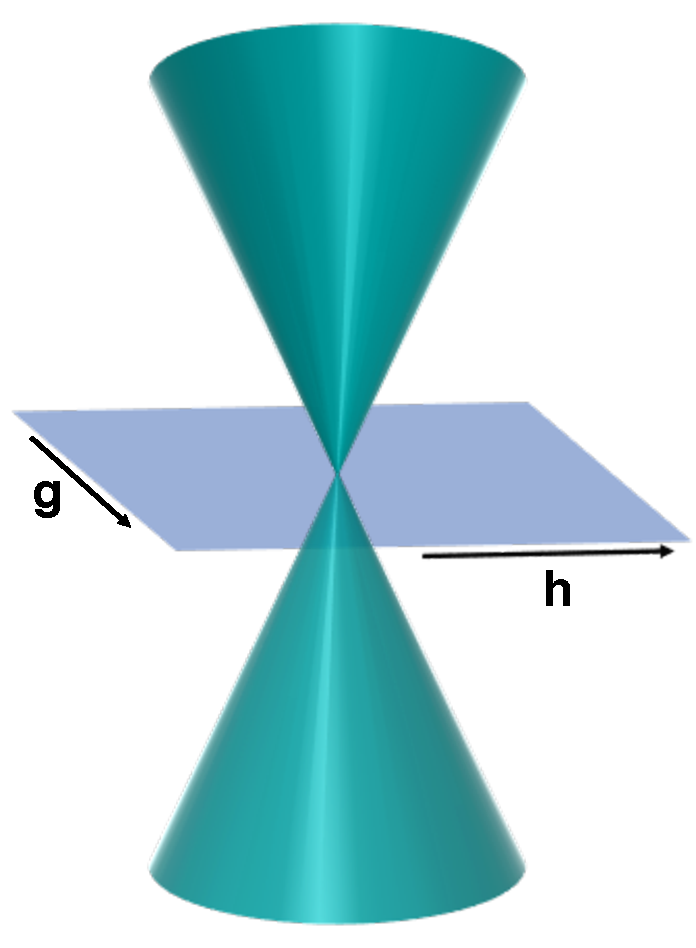
\includegraphics[width=0.4\linewidth]{2Theory/cone.pdf}
  \caption{Schematic of the double-cone topology of degenerate electronic states. The gradient difference vector $\bm{g}$ and the nonadiabatic coupling vector $\bm{h}$ define the branching space lifting the degeneracy.}
  \label{figure: Cone}
\end{figure}
Locating conical intersections is important in determining the feasibility of nonradiative decay mechanisms.\cite{Domcke2011} In particular, the \ac{MECI} between the ground and first excited state is a local minimum on the S\textsubscript{1}/S\textsubscript{0} intersection seam and should dominate the transition between the ground and excited state. Various methods exist to locate the geometry of \acp{MECI} for molecular systems have been developed using the gradient difference and nonadiabatic couplings vectors.\cite{Koga1985,Manaa1993,Bearpark1994,Dallos2004,Yarkony2004} 

In the majority of this work, we use the CIOpt algoirthm of Levine, Coe, and Martinez to locate \acp{MECI} for single-reference methods, where the derivative coupling vectors are not required.\cite{Levine2008} In CIOpt, Legrange multipliers are used to find the minimum of the objective function
\begin{equation}\label{equation: CIOpt}
F_{JI}(\bm{R},\sigma{},\alpha{})=\bm{E}_{JI}(\bm{R})+\sigma{}G_{JI}(\Delta{}E_{JI}(\bm{R},\alpha))
\end{equation}
where 
\begin{equation}
    \bm{E}_{JI}(\bm{R})=\frac{E_{I}(\bm{R})+E_{J}(\bm{R})}{2}
\end{equation}
and
\begin{equation}
    \Delta{}E_{JI}(\bm{R})=E_{J}(\bm{R})-E_{I}(\bm{R})
\end{equation}
where $G_{JI}(\Delta{}E_{JI}(\bm{R},\alpha)$ is a penalty function. Equation \ref{equation: CIOpt} minimises the average energy of states $I$ and $J$ with the penalty function penalising any step which increases the energy gap.  $\sigma$ alters the penalty weight whilst $\alpha$ is a smoothing factor. The interfacing of CIOpt with a variety of electronic structure codes allows \acp{MECI} to be located for a variety of quantum chemical methods. 

The topology of conical intersections calculated by different quantum chemical methods has attracted debate in the community.\cite{Levine2006a,Gozem2014,Tuna2015,Lefrancois2017} It has been shown that CASSCF and MS-CASPT2 wavefunctions show the correct double-cone topology and a ``true" conical intersection. However, surfaces obtained with \ac{TDDFT} instead have a linear crossing instead due to there being no nonadiabatic coupling vector.\cite{Gozem2014}. \ac{ADC2} methods also show a linear intersection, whereas \ac{CC}2 surfaces have the correct conical characteristics but are not completely quantitative.\cite{Tuna2015}. Therefore multireference methods are certainly preferable for modelling S\textsubscript{1}/S\textsubscript{0} crossings. However, single-reference methods can provide a qualitative description of the crossings. Dynamics simulations with these methods have shown for multiple systems that \ac{ADC2} and \ac{CC}2 can provide reasonable results.\cite{Gozem2014,Tuna2015} In the case of TDDFT, a careful selection of the functional is required.\cite{Crespo-Otero2014,Barbatti2015} With the computational cost of multireference methods and the sensitivity of their active space, in this work we use a combination of single- and multireference methods, where \acp{MECI} obtained with \ac{TDDFT}, \ac{ADC2}, and \ac{CC}2 methods are compared to those obtained with CASSCF.
\subsection{Methods for Excited States}\label{section: photo_methods}
One of the most popular methods for probing excited states is \acf{TDDFT}, first proposed in 1984 by Runge and Gross, and then extended in 1995 by Casida, TD-DFT is a popular approach for modelling the properties of electronically excited states[66]. The fundamental idea within TDDFT is that the dynamics of a system can be completely described by its time-dependent density. Runge and Gross proved that there is a unique, 1:1 correspondence between time-dependent densities and potentials.\cite{Runge1984}  From the 1:1 correspondence it follows that the time-dependent density is a unique functional of the external potential (and vice versa). The time-dependent Hamiltonian, and thus the wavefunction, are also functionals of the density, allowing the deduction that all physical observables are functionals of the time-dependent density.

The key quantity in determining the time-dependent density in \ac{TDDFT} is the time-dependent \acf{XC} energy. Just as in \ac{DFT}, \ac{TDDFT} requires a suitable approximation of the \ac{XC}-energy. \ac{TDDFT} uses the \ac{XC}-energy from \ac{DFT} and to construct the time-dependent density, in what is known as the adiabatic approximation. The adiabatic approximation assumes that at each moment in time the \ac{XC}-energy depends only on the instantaneous density. Excitations are calculated in \ac{TDDFT} using linear response theory, which probes the response of a system to a weak perturbation.

A well-known failing in \ac{TDDFT} is the poor description of \acf{CT} excitations, where there is minimal orbital between occupied and virtual orbitals involved in a transition. TDDFT is known to underestimate \ac{CT}-excitation energies with \ac{LDA}, \ac{GGA}, and hybrids, since self-interaction means virtual orbital energies are systematically too low in energy. The \ac{RSH} functionals have been shown to mitigate this error for \ac{CT} excitations, with tuned \ac{RSH} functionals showing equivalent performance wave function methods for the prediction of excitation energies.\cite{Stein2009a,Kuritz2011,Kronik2012a} Within the current work, the \ac{RSH} functional $\omega$B97X-D is used in density functional calculations to incorporate these benefits.\cite{Chai2008} 

In addition, approximate \ac{CC} methods are used to calculate excited state properties of molecules, namely the \ac{CC}2 method. The \ac{CC}2 method was formulated in 1995 to approximate CCSD but with $N^{5}$ scaling and provide accurate excitation energies.\cite{Christiansen1995} In \ac{CC}2, the single excitations of CCSD are retained by the double excitations are approximated, with comparable ground state accuracy of MP2. Response functions of \ac{CC}2 provide excitation energies and transition moments, making it a popular method in probing excited-state properties of molecules.\cite{Sneskov2012}

As an alternative but closely related approach, propagator methods are also used to calculate excitation energies and transtion moments. The polarizer propagator introduces the effect of an external field, for instance the absorption of a photon. In the \ac{ADC2}, the polarizer propagator acts on the \ac{MP2} ground state to give excitation energies at similar accuracy but reduced computational cost compared to \ac{CC}2.
\subsection{Dynamics Simulations of Excited State Processes}\label{section: photo_dynamics}
Simulation of the temporal evolution of photoinduced processes is a powerful method for probing excited-state \acp{PES}. Treating both nuclear and electronic motion fully quantum mechanically, with the required nonadiabatic couplings, is unfeasibly expensive for real molecular systems. As with all quantum chemical approaches, approximations are made. To retain the quantum description of the nuclei, specific nuclear modes can be sampled to reduce the dimensionality of theconfiguration space and the associated computational cost. Alternatively, the nuclear motion can be treated classically and allowed to explore the configuration space determined by the electronic \acp{PES}. 

The second approach, \ac{NA-MQC}, shall be used in elements of this thesis using the \ac{TSH} method. The most prominent \ac{NA-MQC} methods are \ac{TSH}, mean-field Ehrenfest, and multiple spawning.\cite{Crespo-Otero2018} In Ehrenfest dynamics, a nuclear trajectory is calculated using a weighted-average of a predefined number of electronic states. In multiple spawning, a series of Gaussian functions describe the nuclear wavepacket propogating on electronic surfaces. In the vicinity of state crossings, more Gaussian functions are spawned to follow each electronic state. In \ac{TSH}, a set of independent trajectories approximate the nuclear propagation, with electronic transitions determined stochastically, most commonly using Tully's fewest-switches alogrithm.\cite{Tully1990} \ac{TSH} is perhaps the mostly used algorithm for simulating \ac{NA-MQC} dynamics.



\chapter[Nonradiative Decay Mechanisms in 2'-hydroxychalcones]{Nonradiative Decay Mechanisms\\ in 2'-hydroxychalcones}
\label{chapter:NRdecay}
\section{Introduction}\label{section: NRdecay_intro}
Theoretical calculations have the potential to explain the intriguing luminescence properties of the \acf{HC} derivatives introduced in Section \ref{section: lom HC}. \textbf{HC} derivatives \textbf{1}-\textbf{5} of Figure \ref{figure: HC_experimental} have strikingly different emission characteristics in the solid state, for which we wish to disentangle the intra- and intermolecular contributions. This chapter addresses the intramolecular interactions present in the five systems. The effect of the substituents on the four level \ac{ESIPT} photocycle are analysed through a combination of static and nonadiabatic dynamics simulations, investigating the relaxation mechanisms and the competition between different deactivation channels. These simulations show that a strong electron donating group (EDG) in the \textit{para} position alters the topology of the potential energy surface (PES), destabilising the \Estar state, assisting and accelerating proton transfer. Our results provide detailed understanding into the fundamental relaxation mechanisms of \ac{HC}s and the role of the substituents, which is the initial step to unravel the effect of aggregation on the emission properties.

This work presented in this chapter was published in reference\citenum{Dommett2017}. The structure of this chapter follows that of the published article. The computational methods used shall be described, followed by analysis of the vertical excitations, minima on the excited state, and the feasible relaxation channels. Finally the results of nonadiabatic dynamics rationalise those obtained in static calculations. The relevant Supporting Information of ref.\citenum{Dommett2017} is incorporated into the chapter and designated appendices.

\section{Computational Methods}\label{section: NRdecay_methods}
The ground state geometries of all the compounds were optimised in vacuum using resolution of identity \acf{MP2} with the def2-SV(P) and def2-TZVP basis sets.\cite{Haase1993,Schafer1992,Weigend2005} Vertical excitation energies were calculated in vacuum using coupled cluster to approximated second order (\ac{CC}2) and \acf{ADC2} methods under the resolution of identity approximation.\cite{Christiansen1995,Hattig2000,Hattig2002,Kohn2003,Hattig2005} Core electrons were frozen for all \ac{MP2}, \ac{ADC2} and \ac{CC}2 calculations. The performance of the ADC(2) and CC2 methods is compared, whilst the effect of the basis set in the considered for ADC(2). 

Geometry optimisation in the first excited state was carried out in vacuum for \textbf{1}-\textbf{5} with ADC(2) and CC2 methods using the same basis sets as the ground state optimisation. These calculations were performed with Turbomole v7.0.\cite{Turbomole} The level of theory considered to discuss the features of the surfaces is CC2/def2-TZVP, unless otherwise is specified.

The CIOpt software package of Levine, Coe and Martinez was used to determine the location of the \acf{MECI} structures.\cite{Levine2008} The MECI structures were obtained for \textbf{1}-\textbf{5} at the CC2/def2-TZVP, ADC(2)/def2-TZVP, and ADC(2)/def2-SV(P) levels of theory  with $\alpha$=0.02 Hartree. In the case of \textbf{1}, \ac{CAS}\ac{SCF} calculations were performed with MOLPRO program.\cite{Molpro} The \sone/\szero{} conical intersections were optimised with state-averaged CASSCF (SA-CASSCF). The active space considered 12 electrons in 11 orbitals (CASSCF(12,11)) including 2 states in the average with the 6-31G(p) basis set. For the keto \sone/\szero{} \ac{MECI}, the CASSCF(14,13) active space was also considered. The active space is given in Appendix . 
The \acp{PES} were explored through \ac{LIIC} pathways with ADC(2)/def2-TZVP level of theory. In the case of \textbf{1}, the intermediate \ac{LIIC} geometries were relaxed with the $\theta_{tor}$ angle fixed at the CC2/def2-TZVP level of theory. The geometries along the intersection seam were located using CIOpt. 

The absorption spectra of \textbf{1}-\textbf{5} were simulated using the nuclear ensemble method. 500 nuclear configurations were generated based on a Wigner distribution of the harmonic frequencies calculated at MP2/def2-SV(P) level of theory.\cite{Crespo-Otero2012} Five excited states at ADC(2)/def2-SV(P) level of theory were calculated for each individual geometry. For \textbf{1} and \textbf{5}, \acf{TSH} non-adiabatic dynamics simulations were performed using NEWTON-X interfaced with Turbomole, at ADC(2)/def2-SV(P).\cite{Barbatti2014} The initial conditions were generated from the absorption spectra considering an energy window of $\pm$ \si{0.15} {eV} in the absorption spectra, simulating laser excitation.\cite{Barbatti2007} The geometries contributing to these energy windows were used as initial for the trajectory propagation along with their velocities and momenta. \szero{}, \sone{}, and \stwo{} states were included in the dynamics. 

For compound \textbf{1}, an energy window at absorption maximum of 3.35 $\pm$ 0.15 eV was selected for the nonadiabatic dynamics. 50 trajectories were statistically distributed between \sone{} (30) and \stwo{} (20), according to their oscillator strengths. The same protocol was used for compound \textbf{5}, with 50 trajectories (\sone: 30 and \stwo: 20) from an energy window of 3.39 $\pm$ 0.15 eV. The maximum simulation time was 500 fs, with a time step of 0.5 fs and the quantum equations were integrated with 0.025 fs using interpolated quantities between classical steps. Non-adiabatic effects were included using the fewest-switches surface hopping algorithm with decoherence corrections (0.1 Hartree). Non-adiabatic couplings between \stwo{} and \sone{} were estimated approximately using an approximated wave-function and the numerical method.\cite{Ryabinkin2015} The trajectories were terminated when the energy gap between \sone{} and \szero{} was less than 0.1 eV.

\section{Results}\label{section: NRdecay_Results}

\subsection{Vertical Excitations}\label{section: NRdecay_VE}
The vertical excitation energies for the first three excited states were calculated for structures \textbf{1}-\textbf{5} and are summarised in  Table \ref{table: HC_VEs}. Using CC2/def2-TZVP as reference, it is evident that the behaviour of \textbf{5} is somewhat different to \textbf{1}-\textbf{4}. In \textbf{1}-\textbf{4}, there is negligible substituent effect, with a bright \pipistar state predicted for \sone{}, where the energy varies by less than 0.05 eV across the four structures. \stwo{} is a dark \npistar state involving the carbonyl nonbonding pair, whilst \sthree{} is also a dark \pipistar excitation. In compound \textbf{5}, the first two excited states are \pipistar with a red shift of 0.17 eV compared to \textbf{1}, with the oscillator strength of \stwo{} increased at the expense of \sone{}, with the \npistar state shifted to \sthree{}. 

The electron density difference maps between \sone{} and \szero{}, Figure \ref{figure: HC_Vac_Densities},  reveal the origin of differing excitation pattern in \textbf{5}. For \textbf{1}-\textbf{4}, the excitation to \sone{} involves density transfer from the unsaturated bridge of the system (connecting the phenol and dimethylaniline rings) to the carbonyl \pistar orbital. For \textbf{5}, electron density is transferred not from the bridge but from the phenol ring, due to the electron-rich conjugation of the methoxy group. Considerable electron density is transferred from the hydroxyl oxygen, increasing the acidity of the proton. The \stwo{} state in \textbf{5} has the same character as \sone{} in \textbf{1}-\textbf{4}. Thus the strong electron donor in \textbf{5} perturbs the electron density with respect to the other four compounds, changing the character of the bright state with a greater electron depletion at the hydroxyl oxygen. This shall be shown to be important in the following sections as we analyse the relaxation in the excited state.
\begin{figure}[H]
\centering
  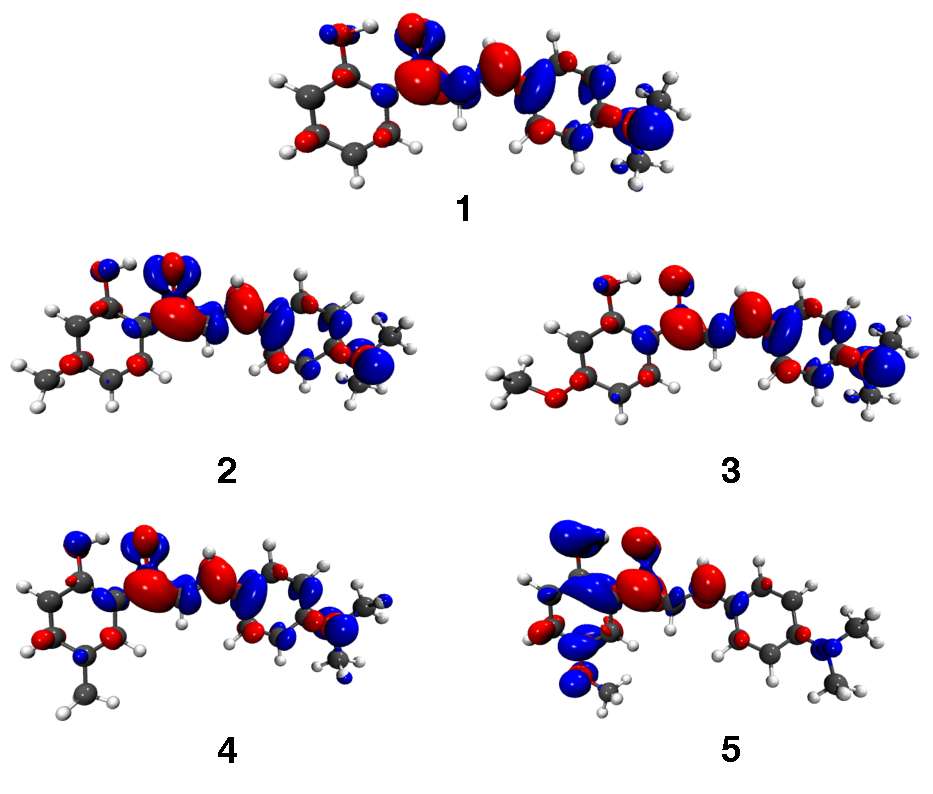
\includegraphics[width=0.8\linewidth]{3nonradiativedecay/HC_Vac_Densities.pdf}
  \caption[Electron density difference maps]{Electron density difference maps (\sone{}-\szero{}) for \textbf{1}-\textbf{5}, showing electron density loss in the ground state (blue) and gain in the excited state (red), calculated at CC2/def2-TZVP level of theory.}
  \label{figure: HC_Vac_Densities}
\end{figure}

Comparing the performance of ADC(2) and CC2 methods, when the same basis set is used (def2-TZVP), ADC(2) vertical excitation energies are about 0.1 eV deviated to the red with respect to the CC2 values. In the case of ADC(2), the def2-SV(P) basis set shifts the energies to the blue in about 0.1 eV. With this basis set there is mixing of the \sone{} and \stwo{} states, where \stwo{} borrows intensity from \sone{} due to  \pipistar and \npistar mixing.. The simulation of the spectra, Figure \ref{figure: HC_spectra_ADC}, using a Wigner-distributed sample of nuclear configurations at the ADC(2)/def2-SV(P) level of theory shows a red shift of 0.1-0.2 eV due to vibrational broadening. Similar shifts are expected for all levels of theory. 

\begin{figure}[H]
\centering
  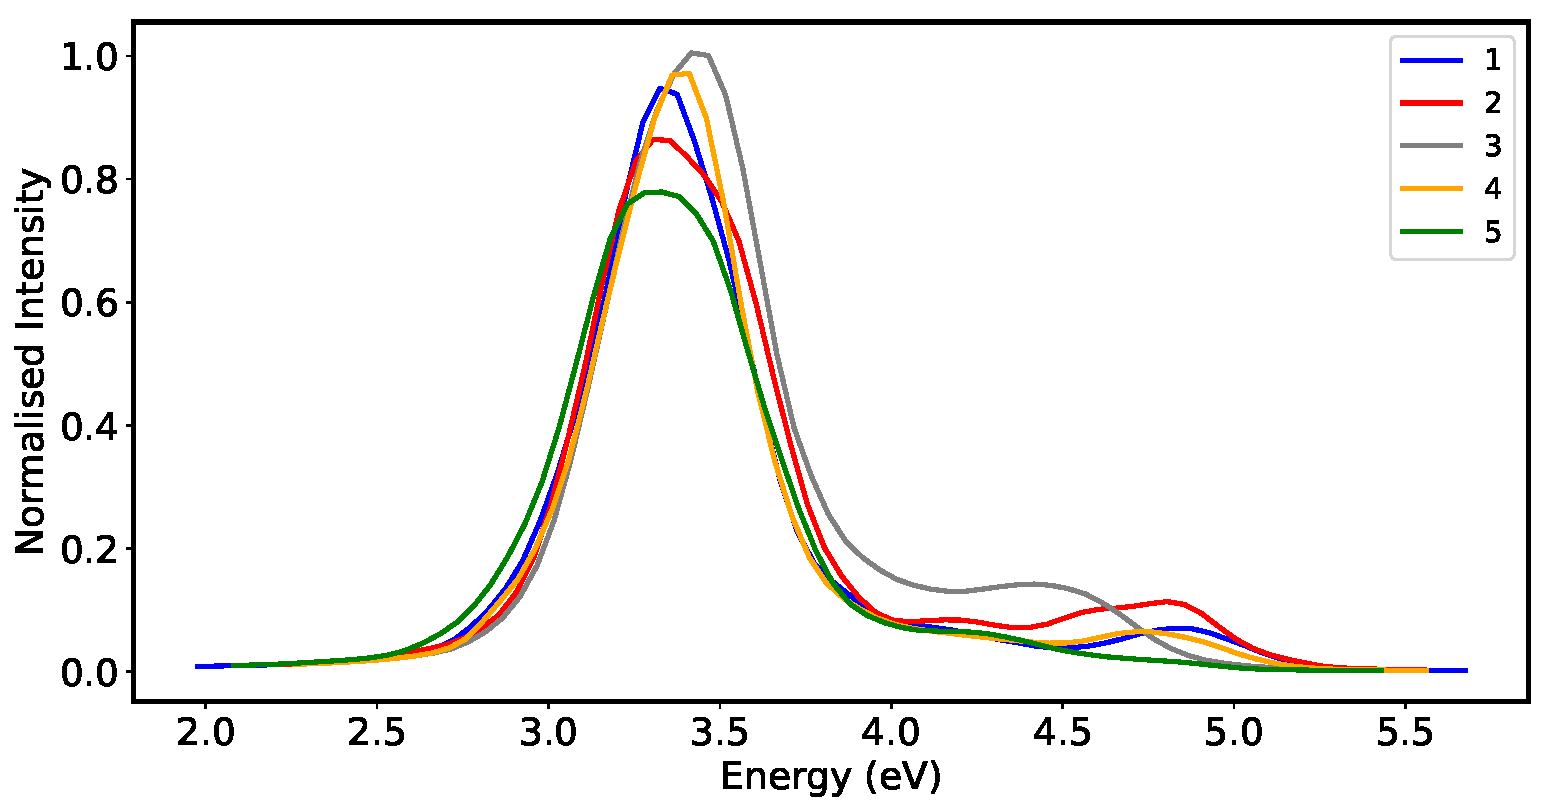
\includegraphics[width=0.8\linewidth]{3nonradiativedecay/HC_Spectra_ADC2.pdf}
  \caption[Simulated absorption spectra of \textbf{HC} \textbf{1}-\textbf{5}]{Simulated absorption spectra of \textbf{HC} \textbf{1}-\textbf{5} at ADC(2)/def2-SV(P) level of theory.}
  \label{figure: HC_spectra_ADC}
\end{figure}

\begin{table}
    \centering
    \begin{tabular}{cccccccccccc}
    \hline
     & \multicolumn{3}{c}{ADC(2)/def2-SV(P)} & & \multicolumn{3}{c}{ADC(2)/def2-TZVP} & & \multicolumn{3}{c}{CC2/def2-TZVP}\\
    \hline
     State & $\Delta$E & \textit{f} & Character & & $\Delta$E & \textit{f} & Character & & $\Delta$E & \textit{f} & Character\\
    \hline
    & \multicolumn{11}{c}{Compound \textbf{1}}\\
     \hline
      \sone   & 3.53 & 0.604 & \pipistar & & 3.36 & 0.869 & \pipistar & & 3.43 & 1.135 & \pipistar\\ 
      \stwo   & 3.58 & 0.391 & \npistar & & 3.44 & 0.090 & \npistar  & & 3.67 & 0.009 & \npistar \\
      \sthree & 3.97 & 0.013 & \pipistar  & & 3.77 & 0.008 & \pipistar & & 3.84 & 0.003 & \pipistar\\ 
      \hline
     & \multicolumn{11}{c}{Compound \textbf{2}}\\
     \hline
     \sone   & 3.53 & 0.483 & \pipistar  & & 3.38 & 0.806 & \pipistar & & 3.43 & 1.167 & \pipistar  \\ 
     \stwo   & 3.59 & 0.551 & \npistar  & & 3.46 & 0.196 & \npistar &  & 3.68 & 0.023 & \npistar \\
     \sthree & 3.96 & 0.010 & \pipistar  & & 3.77 & 0.007 & \pipistar &  & 3.85 & 0.005 & \pipistar \\ 
     \hline
     & \multicolumn{11}{c}{Compound \textbf{3}}\\
     \hline
     \sone   & 3.59 & 1.022 & \pipistar & & 3.40 & 1.063 & \pipistar  &  & 3.47 & 1.286 & \pipistar \\
     \stwo   & 3.64 & 0.075 & \npistar  & & 3.51 & 0.013 & \npistar   &  & 3.75 & 0.002 & \npistar \\
     \sthree & 4.06 & 0.046 & \pipistar & & 3.86 & 0.038 & \pipistar  &  & 3.96 & 0.034 & \pipistar \\ 
      \hline
     & \multicolumn{11}{c}{Compound \textbf{4}}\\
     \hline
     \sone   & 3.53 & 0.404 & \pipistar & & 3.36 & 0.857 & \pipistar &  & 3.42 & 1.105 & \pipistar  \\
     \stwo   & 3.57 & 0.589 & \npistar  & & 3.42 & 0.096 & \npistar  &  & 3.65 & 0.005 & \npistar  \\
     \sthree & 3.86 & 0.002 & \pipistar & & 3.65 & 0.008 & \pipistar &  & 3.72 & 0.028 & \pipistar \\ 
     \hline
     & \multicolumn{11}{c}{Compound \textbf{5}}\\
     \hline
     \sone   & 3.42 & 0.647 &\pipistar & & 3.20 & 0.522 & \pipistar  & & 3.26  & 0.633 & \pipistar  \\
     \stwo   & 3.52 & 0.012 &\npistar  & & 3.39 & 0.066 & \npistar & & 3.54 & 0.390 &  \pipistar\\
     \sthree & 3.67 & 0.337 &\pipistar & & 3.50 & 0.358 & \pipistar & & 3.66& 0.094 &  \npistar \\ 
     \hline
    \end{tabular}
    \caption{Vertical excitation energies, oscillator strengths, and orbital character for compounds \textbf{1}-\textbf{5} at various levels of theory. The corresponding ground state was calculated with the MP2 method with the corresponding basis set. All energies are in eV.}
    \label{table: HC_VEs}
\end{table}


\subsection{Excited State Minima}\label{section: NRdecay_Minima}
Minima in the first excited state for all compounds were optimised using ADC(2) and CC2 methods. The respective energy levels are depicted in Figure \ref{figure: HC_Energy_Levels}. The energy of the \Estar minimum is sensitive to the position and electronic properties of the substituent. An \ac{EDG} in \textit{meta} (\textbf{2} and \textbf{3}) has a negligible effect on the energies of \Estar. However, if the substituent is in \textit{para} (compounds \textbf{4} and \textbf{5}), no stable \Estar minimum can be located. For \textbf{1}-\textbf{3}, relaxation to a local minimum in \Estar is \textit{via} intramolecular rotation. To describe this mode, the torsional rotation angle $\theta_{tor}$ is defined in Figure \ref{figure: H_CC2_LIIC_Scan}.

Two \Estar minima can be found depending on the direction of rotation and in the case of \textbf{1}, both minima are energetically equivalent. For \textbf{1}-\textbf{3}, the energy difference between these minima is very small ($<$ 0.01 eV) and the two minima can be considered degenerate. Torsion through 180\textdegree{} results in cis-trans isomerisation, with the trans isomer about 1 eV less stable than cis in \sone (at ADC(2), Figure \ref{figure: HC_1_Energylevels_ADC2}). Consequently, full cis-trans isomerisation is unlikely. 

For \textbf{1}, the \Estar minimum, $\theta_{tor}$ = 44\textdegree{} and a stabilisation of approximately 0.54 eV with respect to the FC geometry in \sone. Compounds \textbf{2} and \textbf{3} pass through similar minima, with $\theta_{tor}$ = 46\textdegree{} and 54\textdegree{} respectively. Potential energy curves and our non-adiabatic dynamic simulations show that ESIPT from this geometry is improbable. Therefore when occupied the \Estar minimum acts as a sink for the wavepacket to prevent \ac{ESIPT}. The emission energies from the \Estar state for \textbf{1}, \textbf{2} and \textbf{3} are 1.63, 1.59, and 1.46 eV respectively, but with negligible oscillator strength.

In the \Kstar state, where the proton has migrated, the system relaxes \textit{via} intramolecular rotation about $\theta_{tor}$. Two minima with very similar energies can be also located depending on the direction of rotation. The $\theta_{tor}$ value ranges between 40\textdegree{} and 60\textdegree{}. These minima are about 1 eV below the excitation energy corresponding to the FC geometry, and are more stable than \Estar minima. As such a bias towards the ESIPT mechanism can be expected. An \ac{EDG} in \textit{para} (\textbf{4} and \textbf{5}) stabilises the \Kstar \sone{} state with respect to \textbf{1}, but the relative stabilisation with respect the \sone{} energy for the FC geometry is quite similar for all the derivatives (about 1 eV). The emission from \Kstar is in the range of 0.7-1.0 eV for all molecules in \Kstar, but has negligible oscillator strength. \sone{} energies (for \Kstar and \Estar) with ADC(2) method are in good agreement the obtained with CC2 (within the 0.1-0.2 eV range). At the same time, ADC(2) destabilises the K ground state with respect the CC2 method. This behaviour has consequences for the optimisation of MECI and the description of the \sone/\szero{} crossing seam using the ADC(2) method, which are discussed in the next section.

\subsection{Relaxation Channels}\label{section: NRdecay_Channels}
\begin{figure}
\centering
  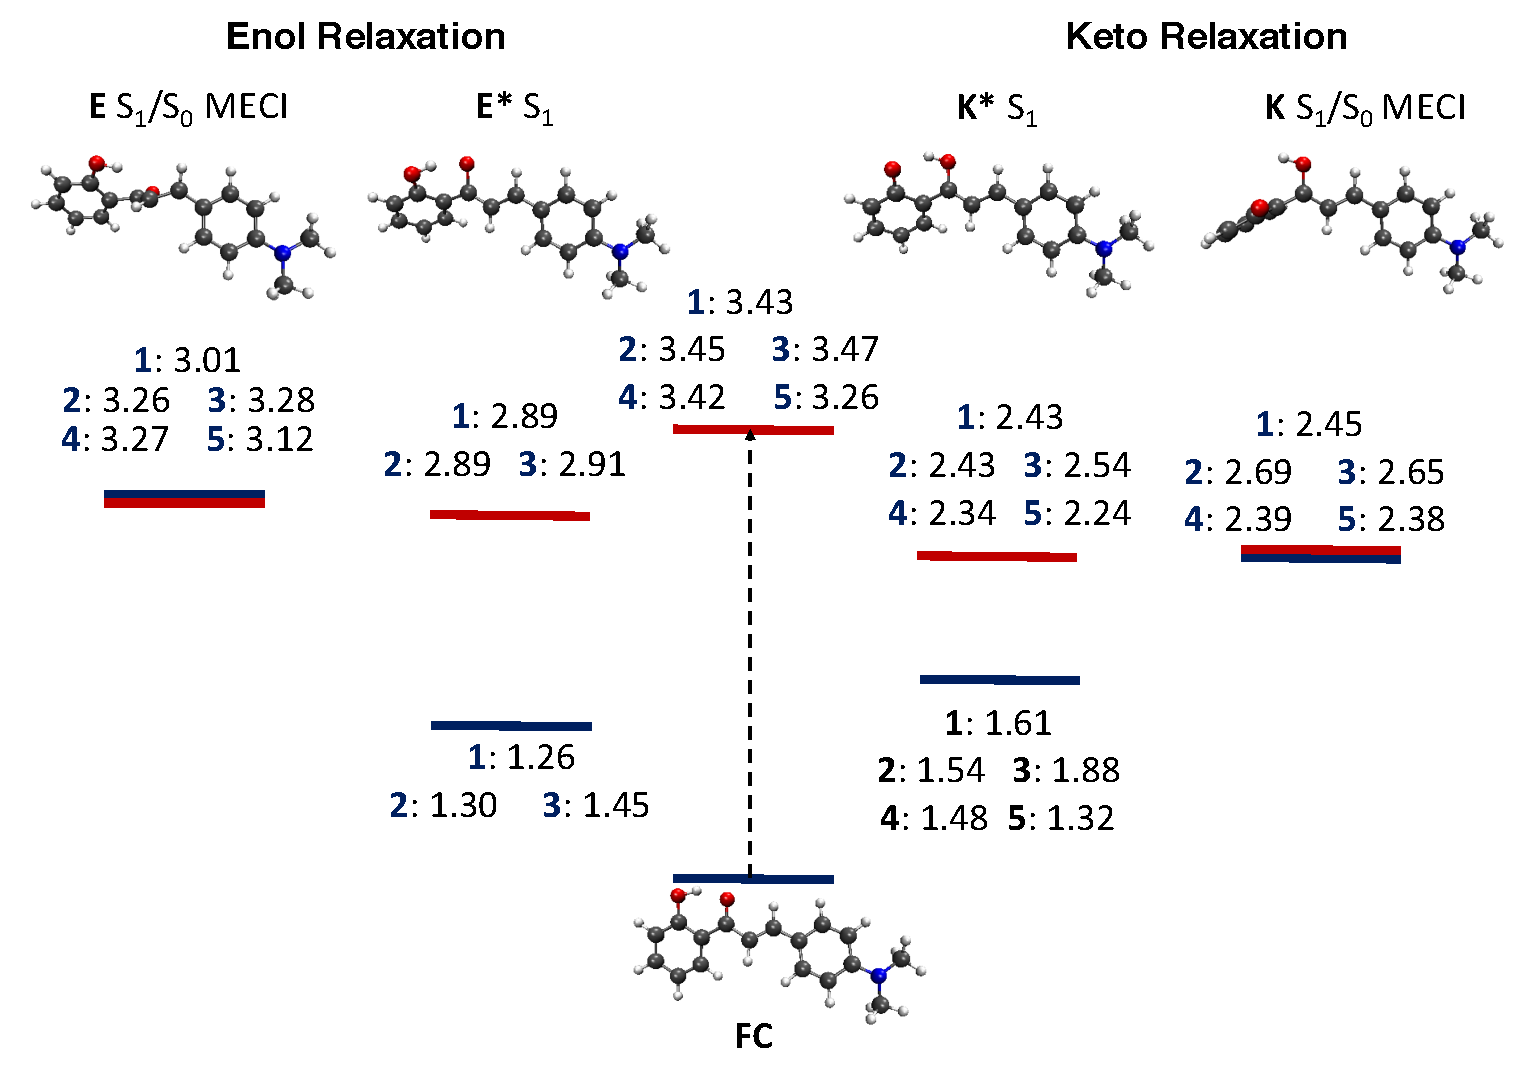
\includegraphics[width=0.9\linewidth]{3nonradiativedecay/HC_Energy_Levels.pdf}
  \caption[\textbf{HC} energy levels]{Relative energies (in eV) for all derivatives calculated at CC2/def2-TZVP level of theory. In all cases, the energy of the ground state was taken as reference.}
  \label{figure: HC_Energy_Levels}
\end{figure}
From the Franck-Condon state, the wavepacket can relax through the enol channel to the \Estar minimum, or the ESIPT channel to the \Kstar minimum. These two competing channels are depicted in Figure \ref{figure: HC_Energy_Levels}. In each channel, the \ac{MECI} was located to determine the feasibility of nonradiative decay \textit{via} a nonadiabatic crossing. For \textbf{1}, the \ac{MECI} geometries were optimised with CC2 methods using the def2-SV(P) and def2-TZVP basis sets. For comparison, the conical intersections were also located with CASSCF(12,11)/6-31G(d) and CASSCF(14,13) levels of theory. The geometry of the \Kstar \sone/\szero{} \ac{MECI} obtained with the CC2 method is in very good agreement with that obtained with CASSCF, $\theta_{tor}$=88\textdegree{} (89\textdegree{} with CASSCF method). The RMSD deviation between the two geometries is just 0.08 \AA. The geometries obtained with both basis sets are very similar. 

For \textbf{1}, the MECI lies at only 0.02 eV above the \Kstar minimum, whilst the substituents slightly increase the energy of the MECI (0.1-0.2 eV) in \textbf{2}-\textbf{5}. Nevertheless, the MECIs remain accessible during the relaxation.  To determine if any barriers exist between the \Kstar minimum and the MECI, we optimise the intermediate states of a linear interpolated pathways, fixing $\theta_{tor}$, at CC2/def2-TZVP level of theory for \textbf{1}. This is shown in Figure \ref{figure: H_CC2_LIIC_Scan}. At the \Kstar minimum, $\theta_{tor}$ = 50\textdegree, and further 30\textdegree{} rotation takes the molecule to the intersection seam. In this region of the potential energy surface, the \sone{} energy does not change significantly with $\theta_{tor}$, which can be associated with an extended crossing seam as previously described by Robb \textit{et al}. in an analogous ESIPT system.\cite{Paterson2005}

\begin{figure}[H]
\centering
  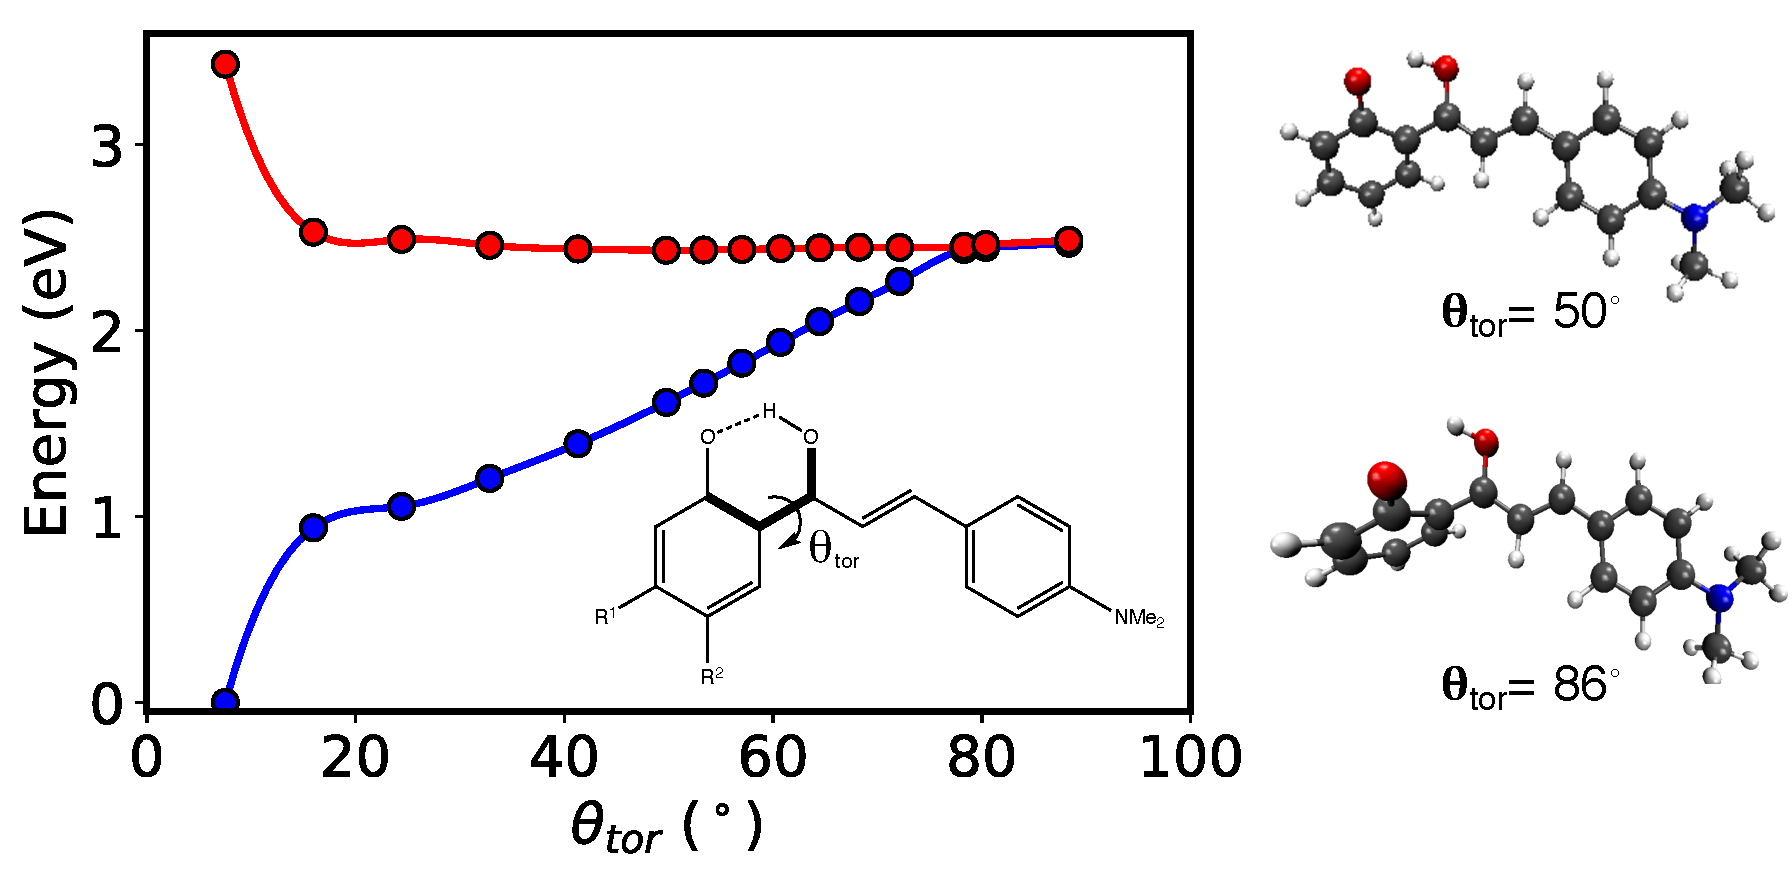
\includegraphics[width=0.9\linewidth]{3nonradiativedecay/H_CC2_LIIC_Scan.pdf}
  \caption[Potential energy surface along the relaxation mode $\theta_{tor}$]{Relaxed linear interpolation pathway between the FC state and the MECI. LIIC located six geometries between the FC state  \Kstar minimum, followed by LIIC to locate 10 geometries between the \Kstar minimum and MECI. All geometries were relaxed at CC2/def2-TZVP level of theory with $\theta_{tor}$ fixed.}
  \label{figure: H_CC2_LIIC_Scan}
\end{figure}

The frustration of intramolecular rotation in the solid state has been hypothesised to prevent access to a conical intersection, resulting in \ac{AIE}. We observe similar results when the dihedral angle is fixed during \Kstar optimisation. The linear interpolation potential energy curves show that there is a stable \Kstar region for \textbf{1} prior to the conical intersection, where emission could take place in the NIR region if the rotation is strongly hindered. The driving force behind the rotation is potentially the stabilisation of the dipole moment, which increases from 7.73 (\szero{}) to 13.32 D (\Estar) upon excitation. This is reduced to 3.99 D in the twisted conformation.

The static calculations suggest that the dominant relaxation process involves a proton transfer step followed by rotation about $\theta_{tor}$. ESPIT is facilitated by the \Kstar minimum, which is more stable than \Estar, especially for \textbf{4} and \textbf{5} (EDG in \textit{para}). Experimentally, \textbf{4} and \textbf{5} do not show fluorescence either in solution or solid state. In the case of the solid state, the lack of fluorescence has been associated with the crystal packing, however these calculations suggest that the character of the substituent might also play a role. This shall be further investigated in the next chapter.

The ADC(2) geometries for the \Kstar \sone/\szero{} MECI of all studied compounds show a $\theta_{tor}$ angle significantly deviated from CC2 and CASSCF values, with the crossing seam reached at a much smaller angle . The ADC(2) MECI structures are very similar to the \Kstar minima (deviated about 10\textdegree{}). This behaviour is associated with the description of the ground state with the MP2 method, which could artificially destabilise \szero{} and thus the \sone/\szero{}  crossing occurs at smaller angles. Similar results were found with def2-SV(P) and def2-TZVP basis sets.

The non-ESIPT relaxation channel is also accessed \textit{via} intramolecular rotation in the \Estar state, leading to a second MECI. The stabilisation of these MECI structures involves relaxation through $\theta_{tor}$, which is significantly larger for \textbf{1} with a value of about 124\textdegree{} (144\textdegree{} with CASSCF). For \textbf{1}, we also observed relaxation through the H-C-C-H dihedral angle (88\textdegree{}). For the rest of the \sone/\szero{} MECI structures (\textbf{2}-\textbf{5}), only $\theta_{tor}$ deviates from the plane. For \textbf{1}-\textbf{3}, the \Estar MECIs are slightly higher in energy than the \Estar minima (0.2-0.3 eV).  Considering the small energy gap and the absence of barriers, the crossing seam region should be accessible. Another mechanism is the direct relaxation to the MECI from the FC geometry, which is the only possibility for \textbf{4} and \textbf{5}, considering the lack of a stable \Estar minimum. These calculations show that the competition between the ESPIT and the relaxation to \Estar will depend on the substituent. While in the case of \textbf{4}-\textbf{5}, a bias towards the ESPIT is expected. Non-adiabatic dynamic simulations confirm this analysis. 
\subsection{Nonadiabatic Dynamics}\label{section: NRdecay_Dynamics}

For these systems, the \sone{} potential energy surfaces obtained with ADC(2) are in a good agreement with the CC2 prior to the conical intersection. The greater computational efficiency of ADC(2) over CC2 also makes it attractive for the study of the first steps of the excited state dynamics of \textbf{HC} systems, although the results when the energy of \szero and \sone converges must be analysed with care. In particular, it is expected that excited state lifetimes may be underestimated.

Compounds \textbf{1} and \textbf{5} represent the extreme cases, with most significant difference in the electronic structure of the excited states. The potential energy surfaces show that rotation around the angle $\theta_{tor}$ is activated during relaxation (\Estar and \Kstar). Surface hopping simulations allow analysis of the competition between different relaxation pathways and the role of rotation in the mechanism. The first steps of the photorelaxation of \textbf{1} and \textbf{5} were explored using non-adiabatic dynamics considering two excited states (\stwo and \sone), which are close in energy.

Our simulations confirm that the main deactivation pathways are associated with relaxation to the \Kstar and \Estar minima. Both mechanisms involve the rotation about $\theta_{tor}$. The competition between both reaction channels strongly depends on the substituent. Figures \ref{figure: HC_1_Populations} and \ref{figure: HC_5_Populations} and show the populations of each adiabatic state as well as the enol and keto population, for \textbf{1} and \textbf{5} respectively. 

\begin{figure}[H]
\centering
  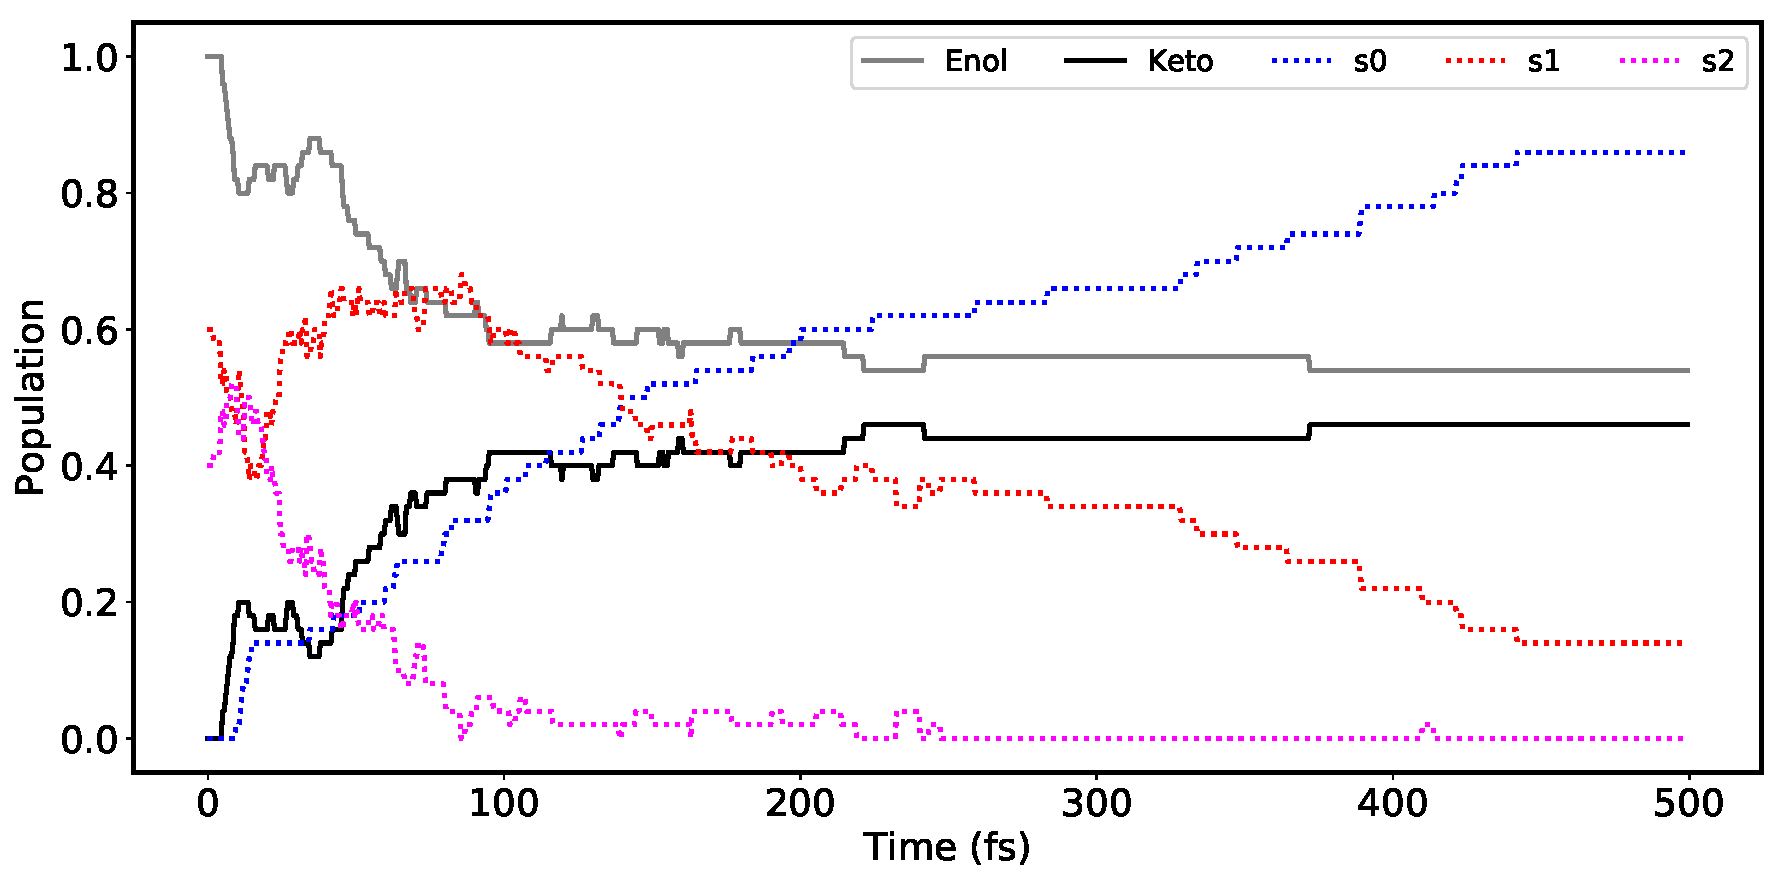
\includegraphics[width=0.9\linewidth]{3nonradiativedecay/HC_1_populations.pdf}
  \caption[Populations of \textbf{HC1} in nonadiabatic dynamics simulations]{The population of the \szero{}, \sone{}, and \stwo{} states for compound \textbf{1} from \ac{TSH} simulations. The population of enol and keto states are also shown.}
  \label{figure: HC_1_Populations}
\end{figure}

In the case of \textbf{1}, both pathways are similarly populated in the dynamics simulations (\Kstar: 48\%, \Estar: 52\%). The population of the different pathways depends on the initial state. For trajectories started in \stwo{}, the fraction is larger (\Kstar: 60\%, \Estar: 40\%). For \textbf{1}, the significant population of the \Estar channel is associated with the stabilisation of the \Estar minimum and the lower acidity of the proton due to the electronic density distribution, as shown in Figure \ref{figure: HC_Vac_Densities}. Conversely, compound \textbf{5} shows a significant preference for the \Kstar channel, with ESIPT occurring in 80\% of trajectories, showing a similar channel preference regardless of the initial state. The methoxy group results in the increased acidity of the proton and lack of stable \Estar minimum, and a heavy bias for the ESIPT channel.
\begin{figure}
\centering
  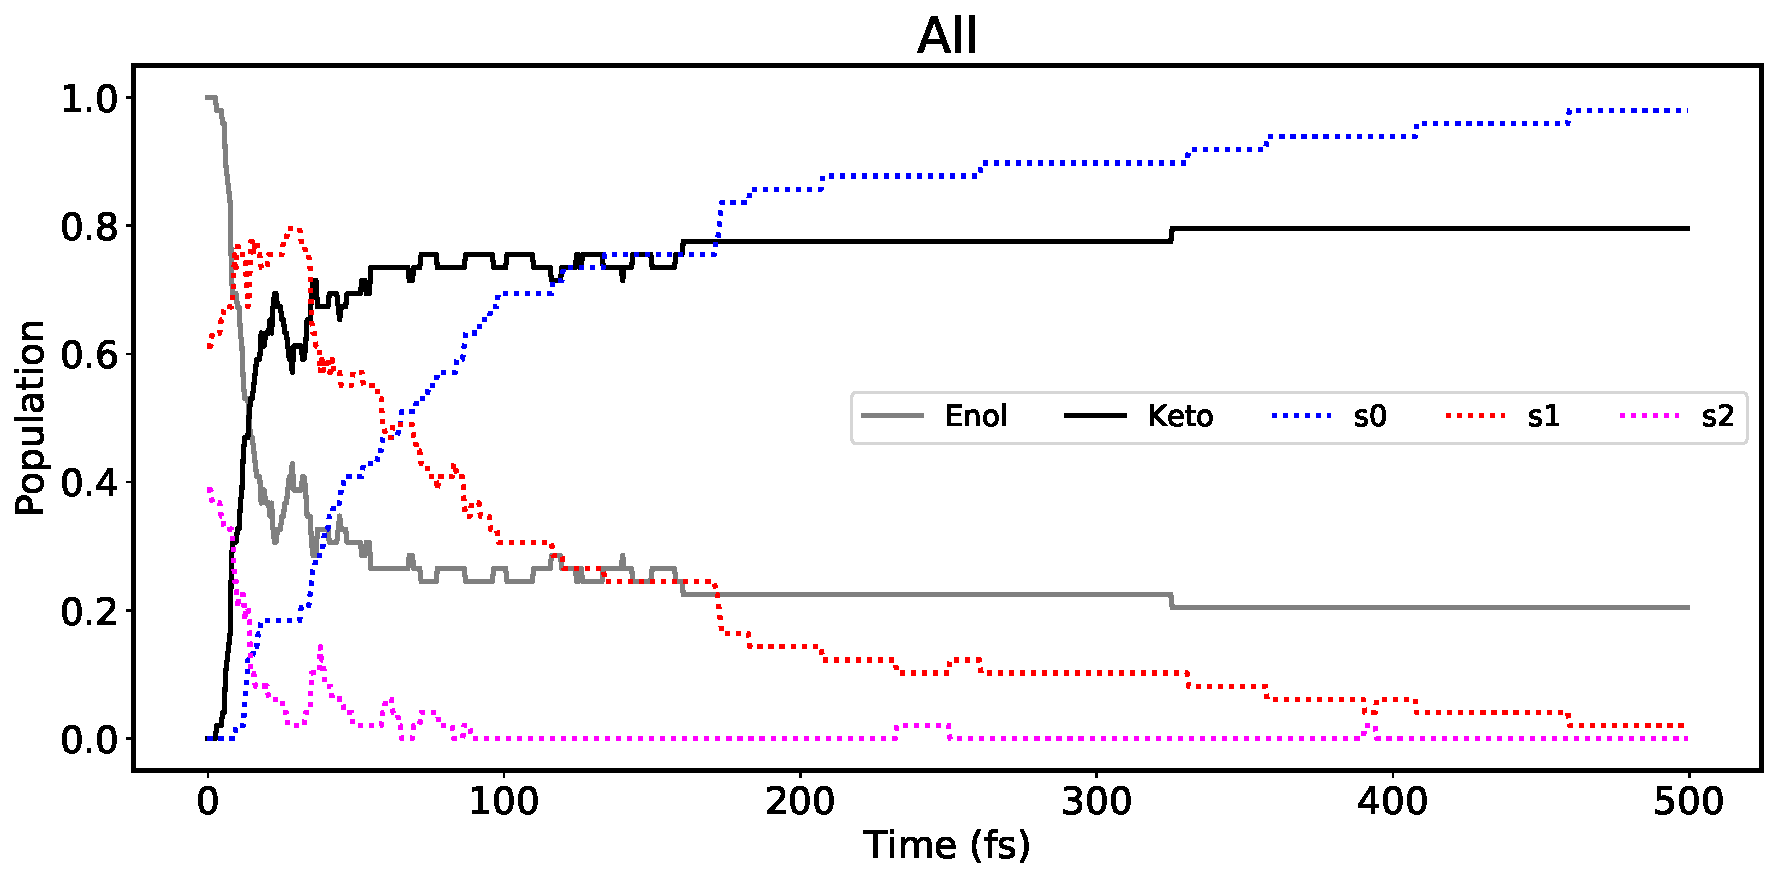
\includegraphics[width=0.9\linewidth]{3nonradiativedecay/HC_5_populations.pdf}
  \caption[Populations of \textbf{HC2} in nonadiabatic dynamics simulations]{The population of the \szero{}, \sone{}, and \stwo{} states for compound \textbf{1} from \ac{TSH} simulations. The population of enol and keto states are also shown.}
  \label{figure: HC_5_Populations}
\end{figure}
The proton transfer time is chosen to be the point at which the proton is equidistant between the phenol and carbonyl oxygens. For \textbf{1} and \textbf{5}, the average time for the first proton transfer is 59 fs and 10 fs respectively, with all trajectories exhibiting ESIPT finding the ground state before the maximum simulation time (500 fs). We identify three steps in the ESIPT mechanism:
\begin{enumerate}
    \item Relaxation in the excited state (\Estar form)
    \item Proton transfer (ESIPT) 
    \item Relaxation in \Kstar followed by internal conversion
\end{enumerate}
These three steps are illustrated for a typical trajectory in panel a) of Figure \ref{figure: HC_1_Trajectories}. During step 1, the angle decreases to $\theta_{tor}$=11\textdegree{} to facilitate the proton transfer in step 2. In some trajectories, the proton oscillates somewhat before transferring. ESIPT in step 2 occurrs at 45 fs. In step 3, the molecule relaxes in the keto form \textit{via} dihedral rotation after which dihedral rotation of 37\textdegree{} results in state convergence after 139 fs, which is underestimated considering the limitations of the ADC(2) method. The region with \sone/\szero{} gap of 0.1 eV is accessed in an average time of 76 fs post-ESPIT for \textbf{1} and 47 fs for \textbf{5}. Considering the features of the PES at ADC(2)/def2-SV(P) level of theory, these times are underestimated with respect to real internal conversion times, but they provide a relative indication of how fast the molecules reach the crossing seam region and the effect of the substituent.
\begin{figure}[H]
\centering
  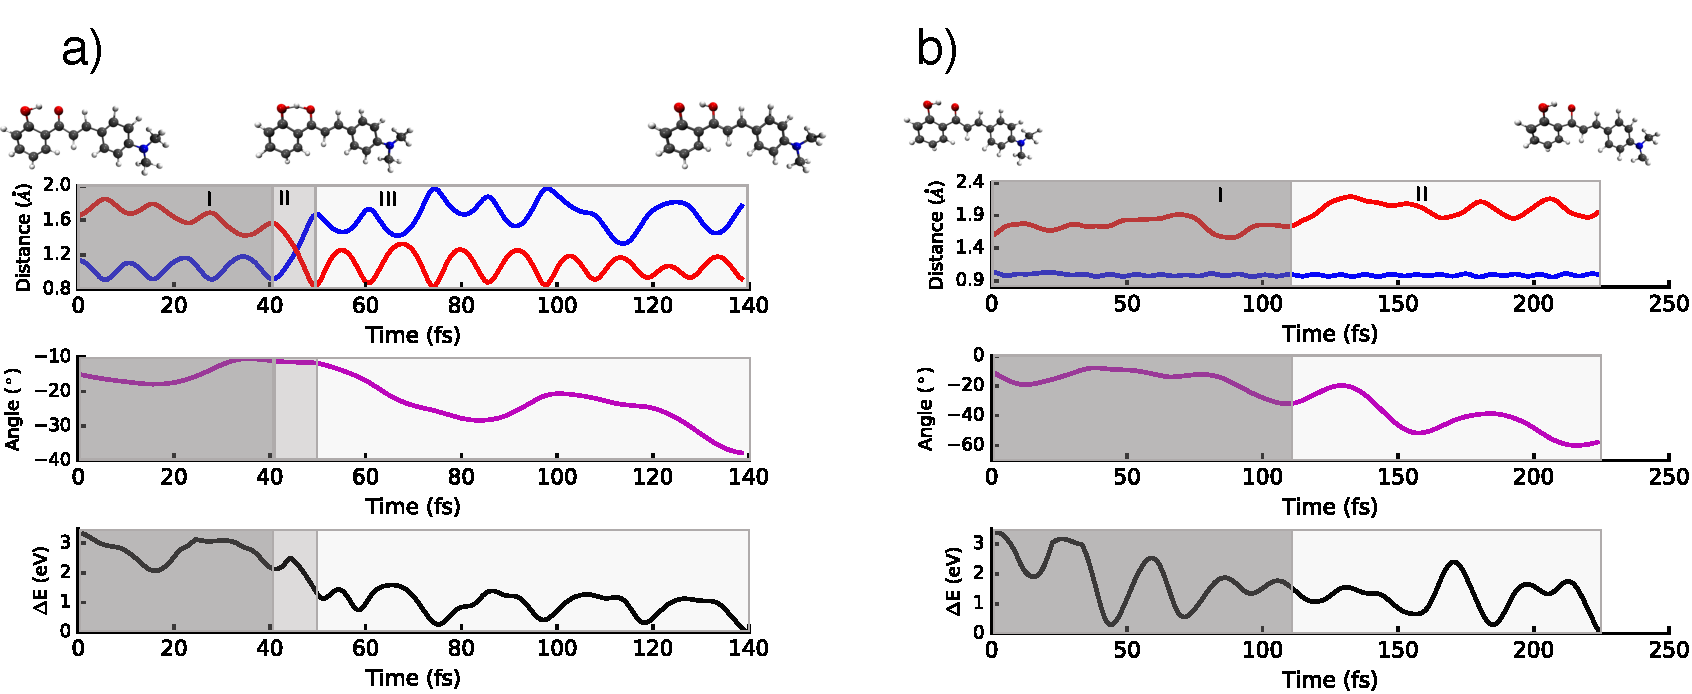
\includegraphics[width=0.9\linewidth]{3nonradiativedecay/HC_1_Trajectories.pdf}
  \caption[Typical trajectories for \textbf{HC1}]{Two exemplar trajectories of compound \textbf{1}. Panel a), left, shows a trajectory undergoing ESIPT, with the associated O-H distances, dihedral angle, and energy gap between \sone{} and \szero{}. The same parameters are shown in panel b) for a trajectory which relaxes in the \Estar channel.}
  \label{figure: HC_1_Trajectories}
\end{figure}

Alternatively to ESIPT, the molecule can remain in the \Estar state. The mechanism of intramolecular rotation in \Estar compromises two steps: 
\begin{enumerate}
    \item Relaxation in the \Estar minimum, which is close to the Franck-Condon geometry.
    \item Further relaxation leading to the internal conversion
\end{enumerate}
Both processes involve the rotation around the angle $\theta_{tor}$. Only 20\% of the trajectories deactivated through this channel did not reach the crossing region within the simulation time. In the case of \textbf{5}, where there is not a \Estar minimum close to the Franck-Condon geometry, the molecule relaxes directly to the crossing seam region. On average, the crossing region is reached within  228 fs for \textbf{1} and 241 fs for \textbf{5}. 

In panel b) of Figure \ref{figure: HC_1_Trajectories}, a typical trajectory undergoing \Estar relaxation is shown. At 0 fs,  $\theta_{tor}$=-10.5\textdegree{}, and for the first 110 fs of the simulation (step 1), the angle oscillates about the equilibrium value (-11.0\textdegree{} at ADC(2)/def2-SV(P) level of theory). Then, the rotation deviates the phenoxy group from the plane prohibiting ESIPT and the molecule reaches the CI region at 225 fs, with an $\theta_{tor}$=-57.6\textdegree{}. The dynamics support the assertions from the potential energy surfaces that proton transfer from the twisted \Estar form, with a barrier of 1.2 eV, is improbable. Relaxation in \Estar therefore competes with ESIPT in compound \textbf{1} due to the close proximity of a local minimum close to the Franck-Condon geometry. Proton transfer followed by internal conversion is the faster process, with an average time duration of 123 fs, compared to 228 fs for rotation in \Estar.

The nonadiabtic dynamic simulations do not allow the prediction of post-internal conversion behaviour, but the analysis of the PES can help understand the following steps in the mechanisms. Post-ESIPT, two relaxation pathways are possible once the MECI is populated. The first completes the four-level photocycle and returns the system to the ground state cis-enol form \textit{via} \ac{GSIPT}. The second continues the rotation about $\theta_{tor}$ to produce the trans-keto form of \textbf{HC}.  Optimisation at the MP2/def2-TZVP level show this structure is more than 1 eV less stable than the ground state, suggesting that \ac{GSIPT} will be preferential. This is shown schematically in Figure \ref{figure: HC_1_Energylevels_ADC2}. The nonadiabatic dynamics simulations clearly illustrate the effect of a strong electron donor in the \textit{para} position on the ESIPT process in \ac{HC}s. The population of the ESIPT channel and rate of proton transfer is greatly increased as is subsequent convergence of the ground and first excited state. 

\begin{figure}
\centering
  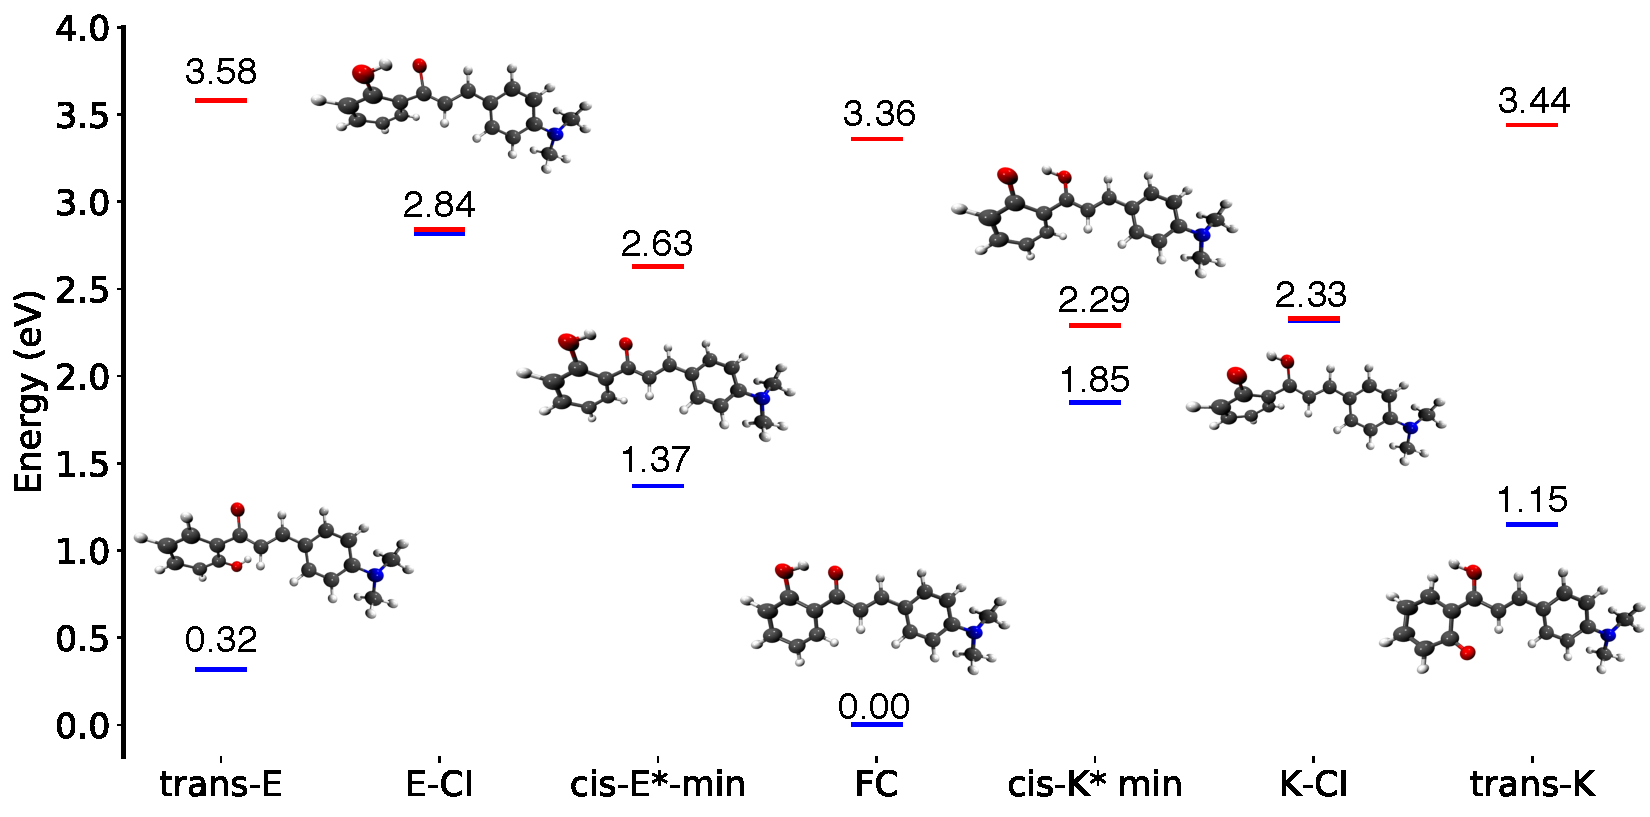
\includegraphics[width=0.9\linewidth]{3nonradiativedecay/HC_1_energylevels_ADC2.pdf}
  \caption[Energies of important optimised energies for \textbf{1}]{Energies of important optimised energies on the \ac{PES} of \textbf{1}. Ground states optimised at MP2/def2-TZVP, whilst excited state minima optimised at ADC(2)/def2-TZVP level of theory.}
  \label{figure: HC_1_Energylevels_ADC2}
\end{figure}

\subsection{Conclusions}\label{section: NRdecay_Conclusions}
In this chapter state-of-the-art computational methods have been applied to investigate the photochemistry of five derivatives of \ac{HC}, an ESIPT-active compound with potential application in organic lasers and optoelectronics. Experimental data show that \ac{HC}s are non-emitting in solution and only fluoresce through \ac{AIE}.\cite{Cheng2015} The calculations provide theoretical description of the ESIPT process and subsequent relaxation mechanisms of \ac{HC}s in gas phase, which represents the first step for the understanding of the photochemistry of these systems. 

Through calculation of vertical excitation energies and corresponding absorption spectra, we find that electron donating groups have but a small influence of the absorption characteristics of \ac{HC}. It takes a strong electron donor in the \textit{para} position to alter the vertical excitation energy, on account of the increased conjugated electron density. On the other hand, relaxation back to the ground state is far more sensitive to the electron donating power of the substituent and its positioning on the phenol moiety. Dual-emission is inhibited with an EDG in \textit{para} for \ac{HC}s. This is quite unexpected, with a comprehensive study on the effects of substituents in common ESIPT-compounds finding that electron donating groups in any position favour the \Estar form, showing the complex nature of ESIPT chromophores.\cite{Azarias2016}

The ground state is accessible \textit{via} non-radiative channels from both \Estar and \Kstar states. \sone/\szero{} MECI structures were found for all compounds, associated with an extended crossing seam. Both mechanisms involve the activation of an intermolecular rotation mode about the $\theta_{tor}$ angle. The competition between both mechanisms depends strongly on the position and nature of the substituent of the substituent. Proton transfer is more favourable with electron donating groups in \textit{para}, correlating with donating power and increased electron density loss at the phenol oxygen. Nonadiabatic surface-hopping dynamic simulations provide a full picture of relaxation energetics and timescales. 

ESPIT is strongly favoured for \textbf{4}-\textbf{5}, where there are not stable \Estar minima. For compound \textbf{5}, the reaction coordinate is completely downhill correlating with intramolecular rotation. The dynamic simulations show a bias towards the \Kstar relaxation mechanism. Experimentally, \textbf{4} and \textbf{5} do not fluoresce either in solution or solid state. Wang et al. suggested that for the solid material, this behaviour is related to the crystal packaging.\cite{Cheng2015} Our calculations show that the character of the substituent and the electronic effects in the monomers might also play a role in the mechanism. Further calculations have been carried out in solid state to confirm this hypothesis, which shall be discussed in the next chapter. 




%\appendix 

\bibliographystyle{rsc}
\bibliography{Thesis}

\end{document}
